\documentclass{article}
\usepackage{graphicx} % Required for inserting images

\title{\Huge FROZEN LAKE'S REINFORCEMENT LEARNING AGENT REPORT}
\author{Francesco Saverio Sconocchia Pisoni 1889241}
\date{March 2025}

    


\begin{document}

\maketitle

\begin{center}
    \centering
    \resizebox{\textwidth}{!}{
\includegraphics{logo Sapienza (rgb).png}}
\end{center}

\section*{\centering ARTIFICIAL INTELLIGENCE AND MACHINE LEARNING 2023/2024}
\clearpage


\section{Introduction}

This machine learning project aims to maximize the average reward taken by solving the Frozen Lake environment, using reinforcement learning techniques.
This technique allows us to reach the goal through a slippery (in this case) obstacle path.
This is done by creating an agent which interfaces with this environment (through the Gymnasium library), collecting a reward and arriving to a new reached state.
The agent is able to calculate and improve an expected reward by taking an action in a state, using the non-deterministic Q-learning method.
After the calculated Q-table is converged to an optimal solution, the agent could solve the environment by choosing the best expected reward action from the Q-table itself.

\begin{center}
\centering
\resizebox{\textwidth}{!}{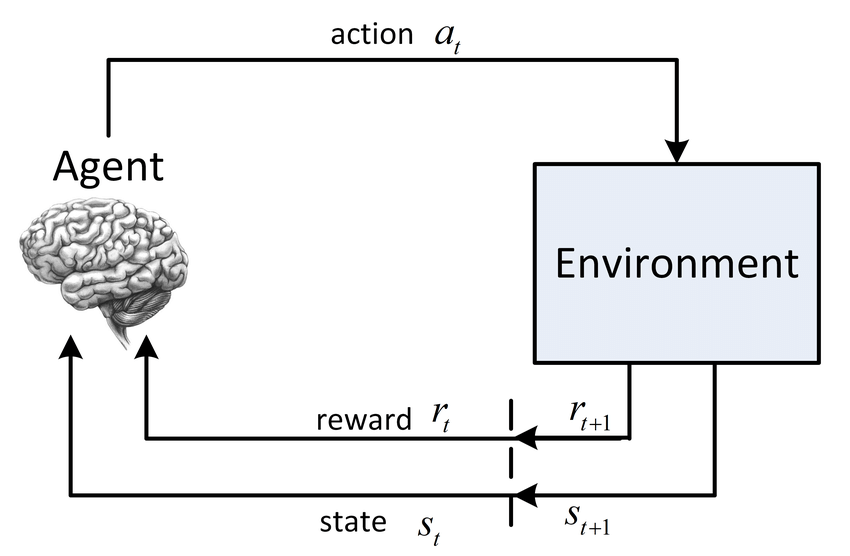
\includegraphics{agent-environment-schema.png}}
\end{center}

We use the non-deterministic method, because of the slippery of the floor of the environment, which could bring (with a certain probability) the agent to find itself in a non-expected state, after performing a chosen action.

The non-deterministic Q-learning method is described below:

\begin{center}
\centering
\resizebox{\textwidth}{!}{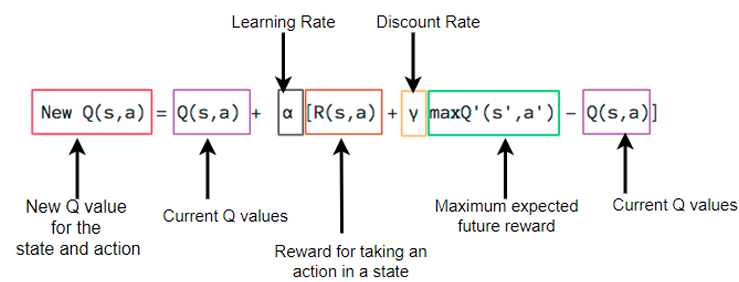
\includegraphics{nd-Q-learning-function.png}}
\end{center}

Is needed to clarify the meaning of those parameters:

\begin{itemize}
\item[--]{Learning rate $\alpha$: it indicates how fast should change the Q-table's parameters in the training phase}
\item[--]{Discount rate $\gamma$: it determines the importance of future rewards}
\item[--] {max Q'(s', a') : it calculates the maximum Q-value among all the possible actions which could be taken from the new reached state s'}
\end{itemize}


\section{Environment}

The Frozen Lake environment has the following characteristics: 
\begin{itemize}
\item[--]{An observation space of 16 possible values, where each possible integer indicates a specific cell of the map, which is the player’s current position and is calculated as current\_row * ncols + current\_col}
\item[--] An action space of 4 possible values, representing the following actions: 0 = Move left, 1 = Move down, 2 = Move right, 3 = Move up
\item[--] The reward could be 1 if the agent reaches the goal, or 0 if not
\item[--] Each episode terminates if the agent reaches the goal or if the agent hits an obstacle (falls in the lake) or if the agent performs more than 100 steps in an episode
\item[--] The slippery characteristic is encoded in this way: the player will move in intended direction with probability of 1/3 else will move in either perpendicular direction with equal probability of 1/3 in both directions.
\end{itemize}

\subsection{Exploration-exploitation}

When the agent, in the training phase, has to choose an action to perform in order to improve its Q-table, we want that it chooses primarily random actions in order to better exploring all the environment and its rewards.
But later on, we want to converge to an optimal solution, which could be reached by using the best actions to be able to achieve the goal.


\subsection{General solution adopted}


My solution for both Deep Q Network and Tabular Q Learning methodologies used for solving the environment uses:
\begin{itemize}
\item[--] A constant learning rate, which converges the same.
\item[--] The Epsilon-greedy strategy : Is chosen either the best action with a probability 1-$\epsilon$ or a random action in the training phase, for managing the duality exploration-exploitation.
\item[--] The epsilon $\epsilon$ parameter decreases linearly with a decay factor, until reaches a minimum value, so achieving first exploration and then exploitation.
\end{itemize}



\section{Tabular Q Learning}

\subsection{Solution adopted}

The agent algorithm has the following characteristics:
\begin{itemize}
\item[--] {A decay function which is called at each episode for decreasing the $\epsilon$ value:
\begin{verbatim}
self.epsilon = max(self.final_epsilon, self.epsilon - self.epsilon_decay)
\end{verbatim}
}
\item[--] In the training phase, a number of episodes of 15.000 episodes
\item[--] In the training phase, a range of 250 episodes for calculating the average cumulative reward over that range of episodes, so limiting the noise
\item[--] In the test phase, a number of 500 episodes
\end{itemize}

\subsection{Metric results}

\subsubsection{Changing the epsilon decay}

These are the common hyper parameters for the runs:
\begin{itemize}
\item[--] $\alpha$= 0.1
\item[--] initial $\epsilon$ = 1
\item[--] final $\epsilon$ = 0.05
\item[--] gamma = 0.99
\end{itemize}

From the first plot to the third, the $\epsilon$ decay rate is increased as follows:
\begin{itemize}
\item[--] The first brings $\epsilon$ to its minimum value at 7/8 of the episodes.
\item[--] The second brings $\epsilon$ to the minimum at 3/4 of the episodes.
\item[--] The last one brings $\epsilon$ to the minimum at 1/2 of the total episodes.
\end{itemize}

\begin{center}
\centering
\resizebox{\textwidth}{!}{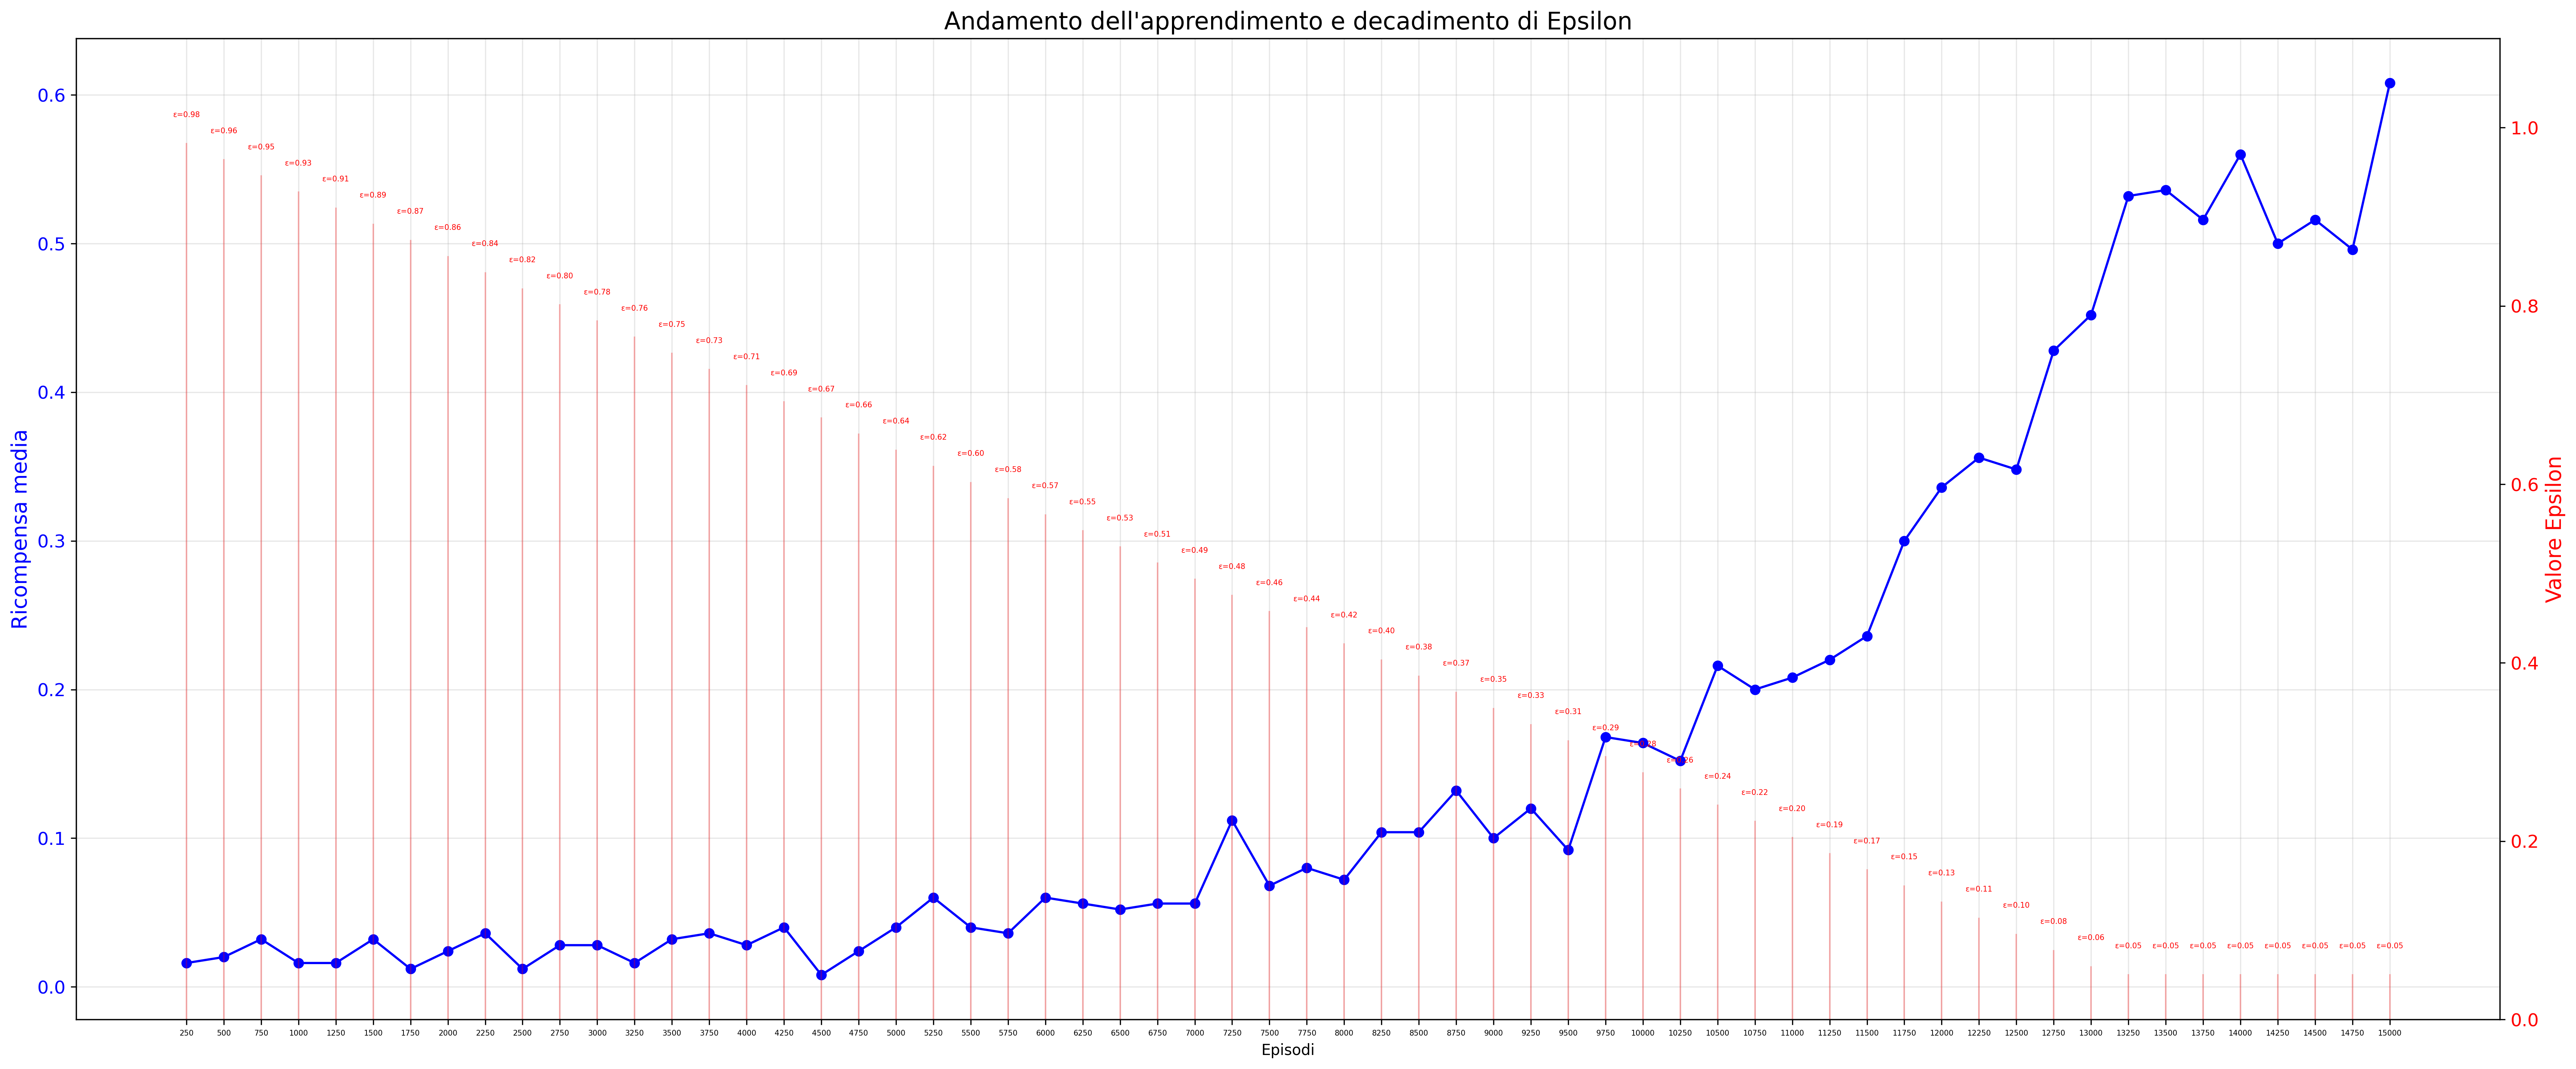
\includegraphics{TQL;lr=0.1;nep=15000;eps=1.0;fineps=0.05;eps_dec=7.238095238095238e-05;gam=0.99.png}}
\end{center}


\begin{center}
\centering
\resizebox{\textwidth}{!}{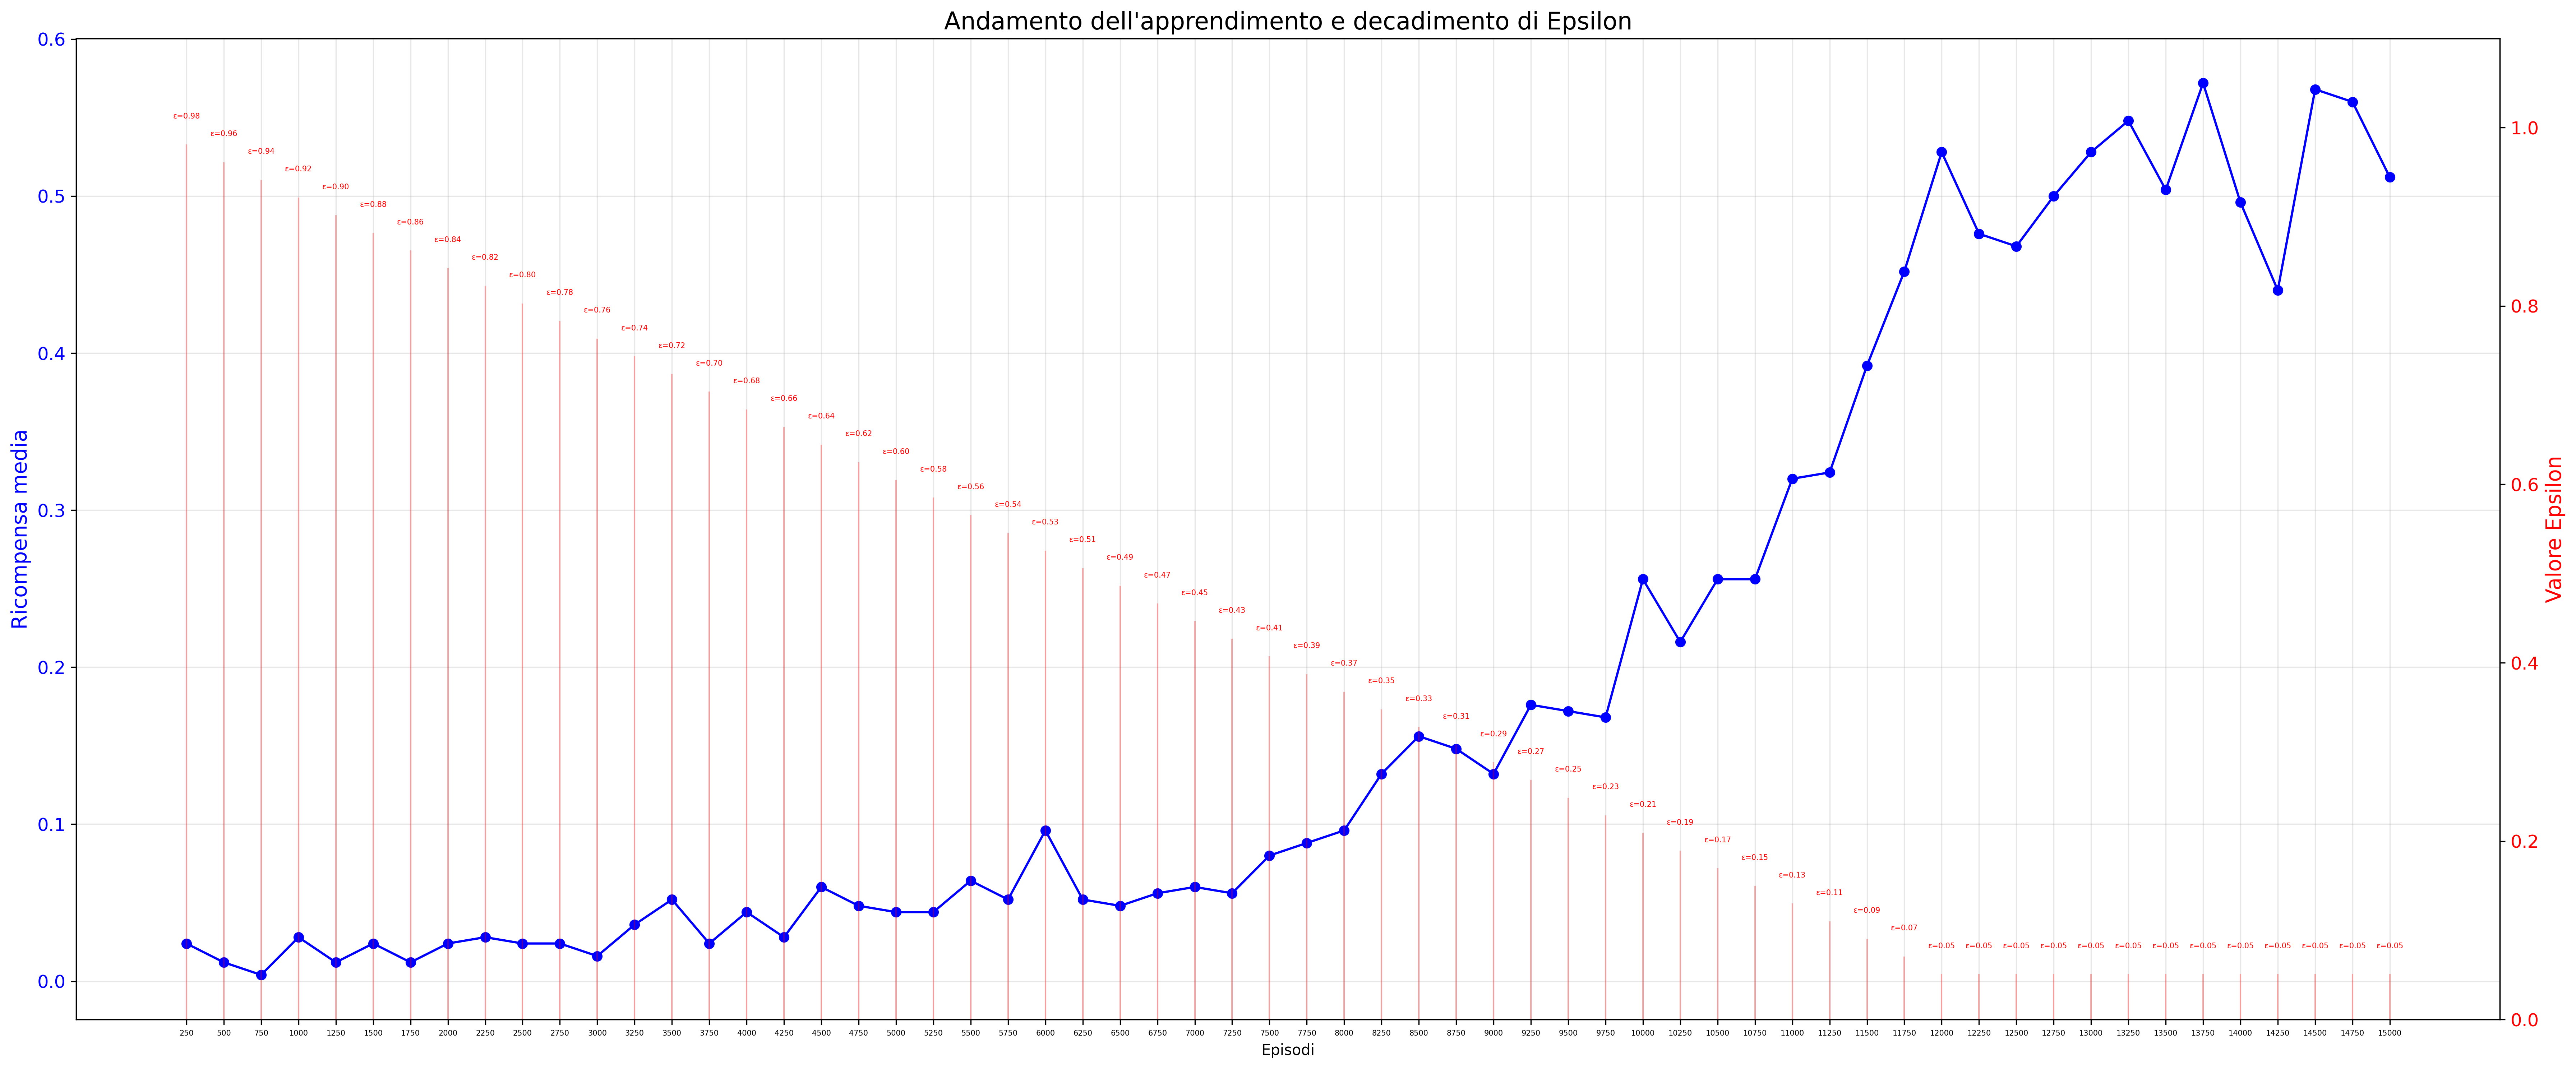
\includegraphics{TQL;lr=0.1;nep=15000;eps=1.0;fineps=0.05;eps_dec=7.916666666666666e-05;gam=0.99.png}}
\end{center}


\begin{center}
\centering
\resizebox{\textwidth}{!}{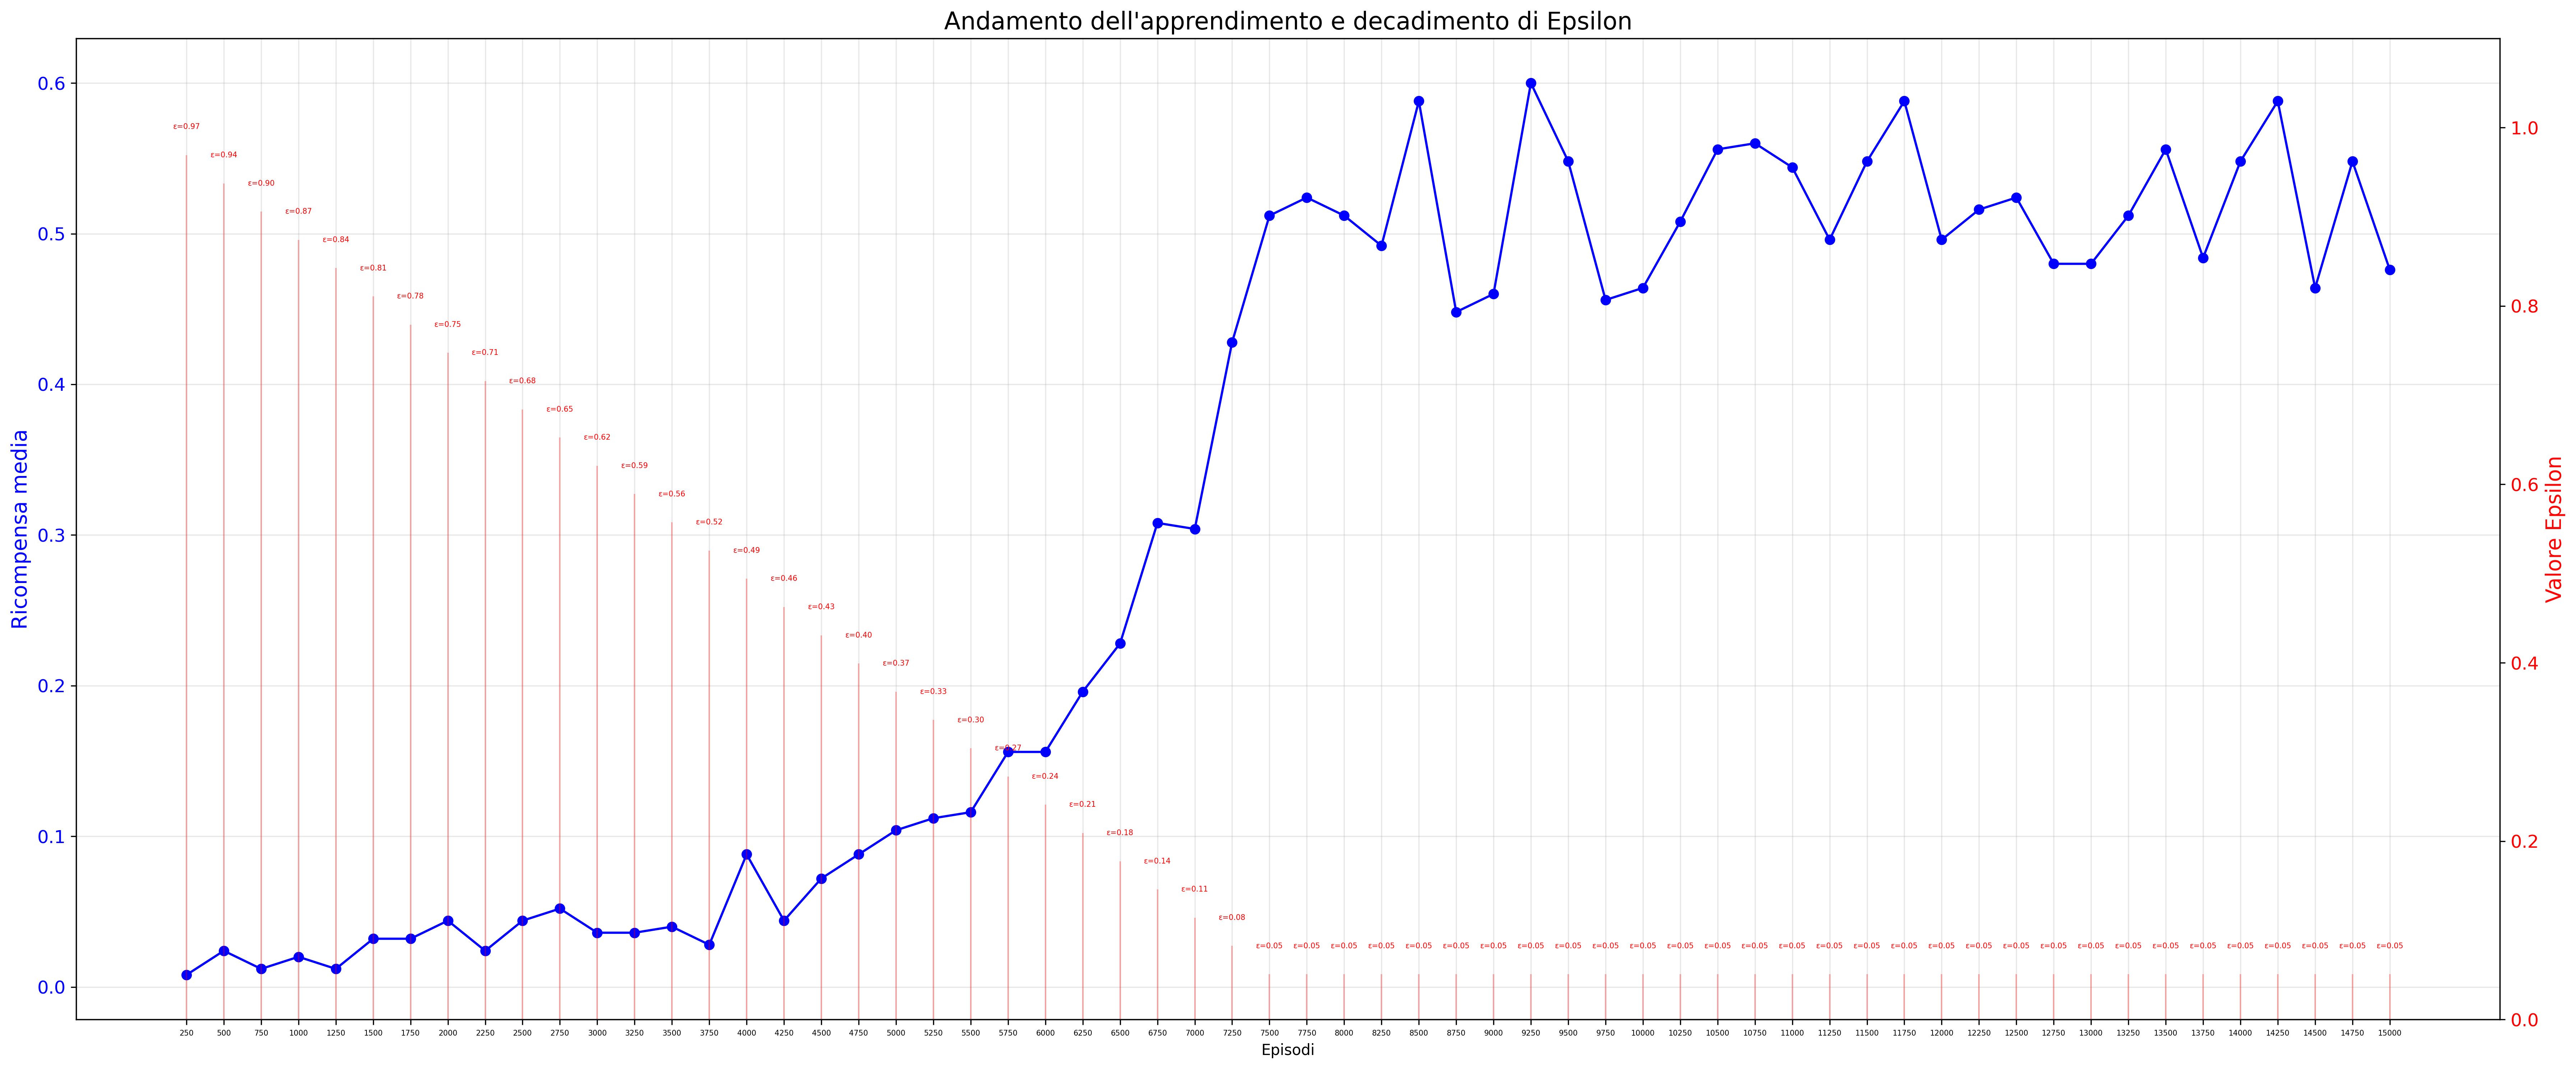
\includegraphics{TQL;lr=0.1;nep=15000;eps=1.0;fineps=0.05;eps_dec=0.00012666666666666666;gam=0.99.png}}
\end{center}

\clearpage


The convergence occurs when $\epsilon$ reaches the minimum value (0.05), so the third setting beats the others in terms of convergence time.
\\
In terms of average cumulative reward at convergence, both the first and the third configurations have roughly the same value (about 55\% success rate). Instead, the second configuration (full exploration at 3/4 of the episodes) results in an average cumulative reward of about 50\%.
\\
During the testing phase, the first configuration achieves a success rate of 73.6\% (over 500 test episodes), while the other two configurations show success rates of 72.8\% for the second one and 72.6\% for the third.
\\
Therefore, we can conclude that the third configuration is the best, due to its faster convergence time, along with one of the best average cumulative rewards at convergence and nearly the same success rate in the test phase as the other configurations.


\subsubsection{Changing the learning rate}

These are the common hyper parameters for the runs:
\begin{itemize}
\item[--] $\epsilon$ decay= 0.000126
\item[--] initial $\epsilon$ = 1
\item[--] final $\epsilon$ = 0.05
\item[--] gamma = 0.99
\end{itemize}

From the first plot to the third, the $\alpha$ value assumes the following values :
\begin{itemize}
\item[--] The first sets $\alpha$ to 0.1
\item[--] The second sets $\alpha$ to 0.01
\item[--] The third sets $\alpha$ to 0.001
\end{itemize}

\clearpage


\begin{center}
\centering
\resizebox{\textwidth}{!}{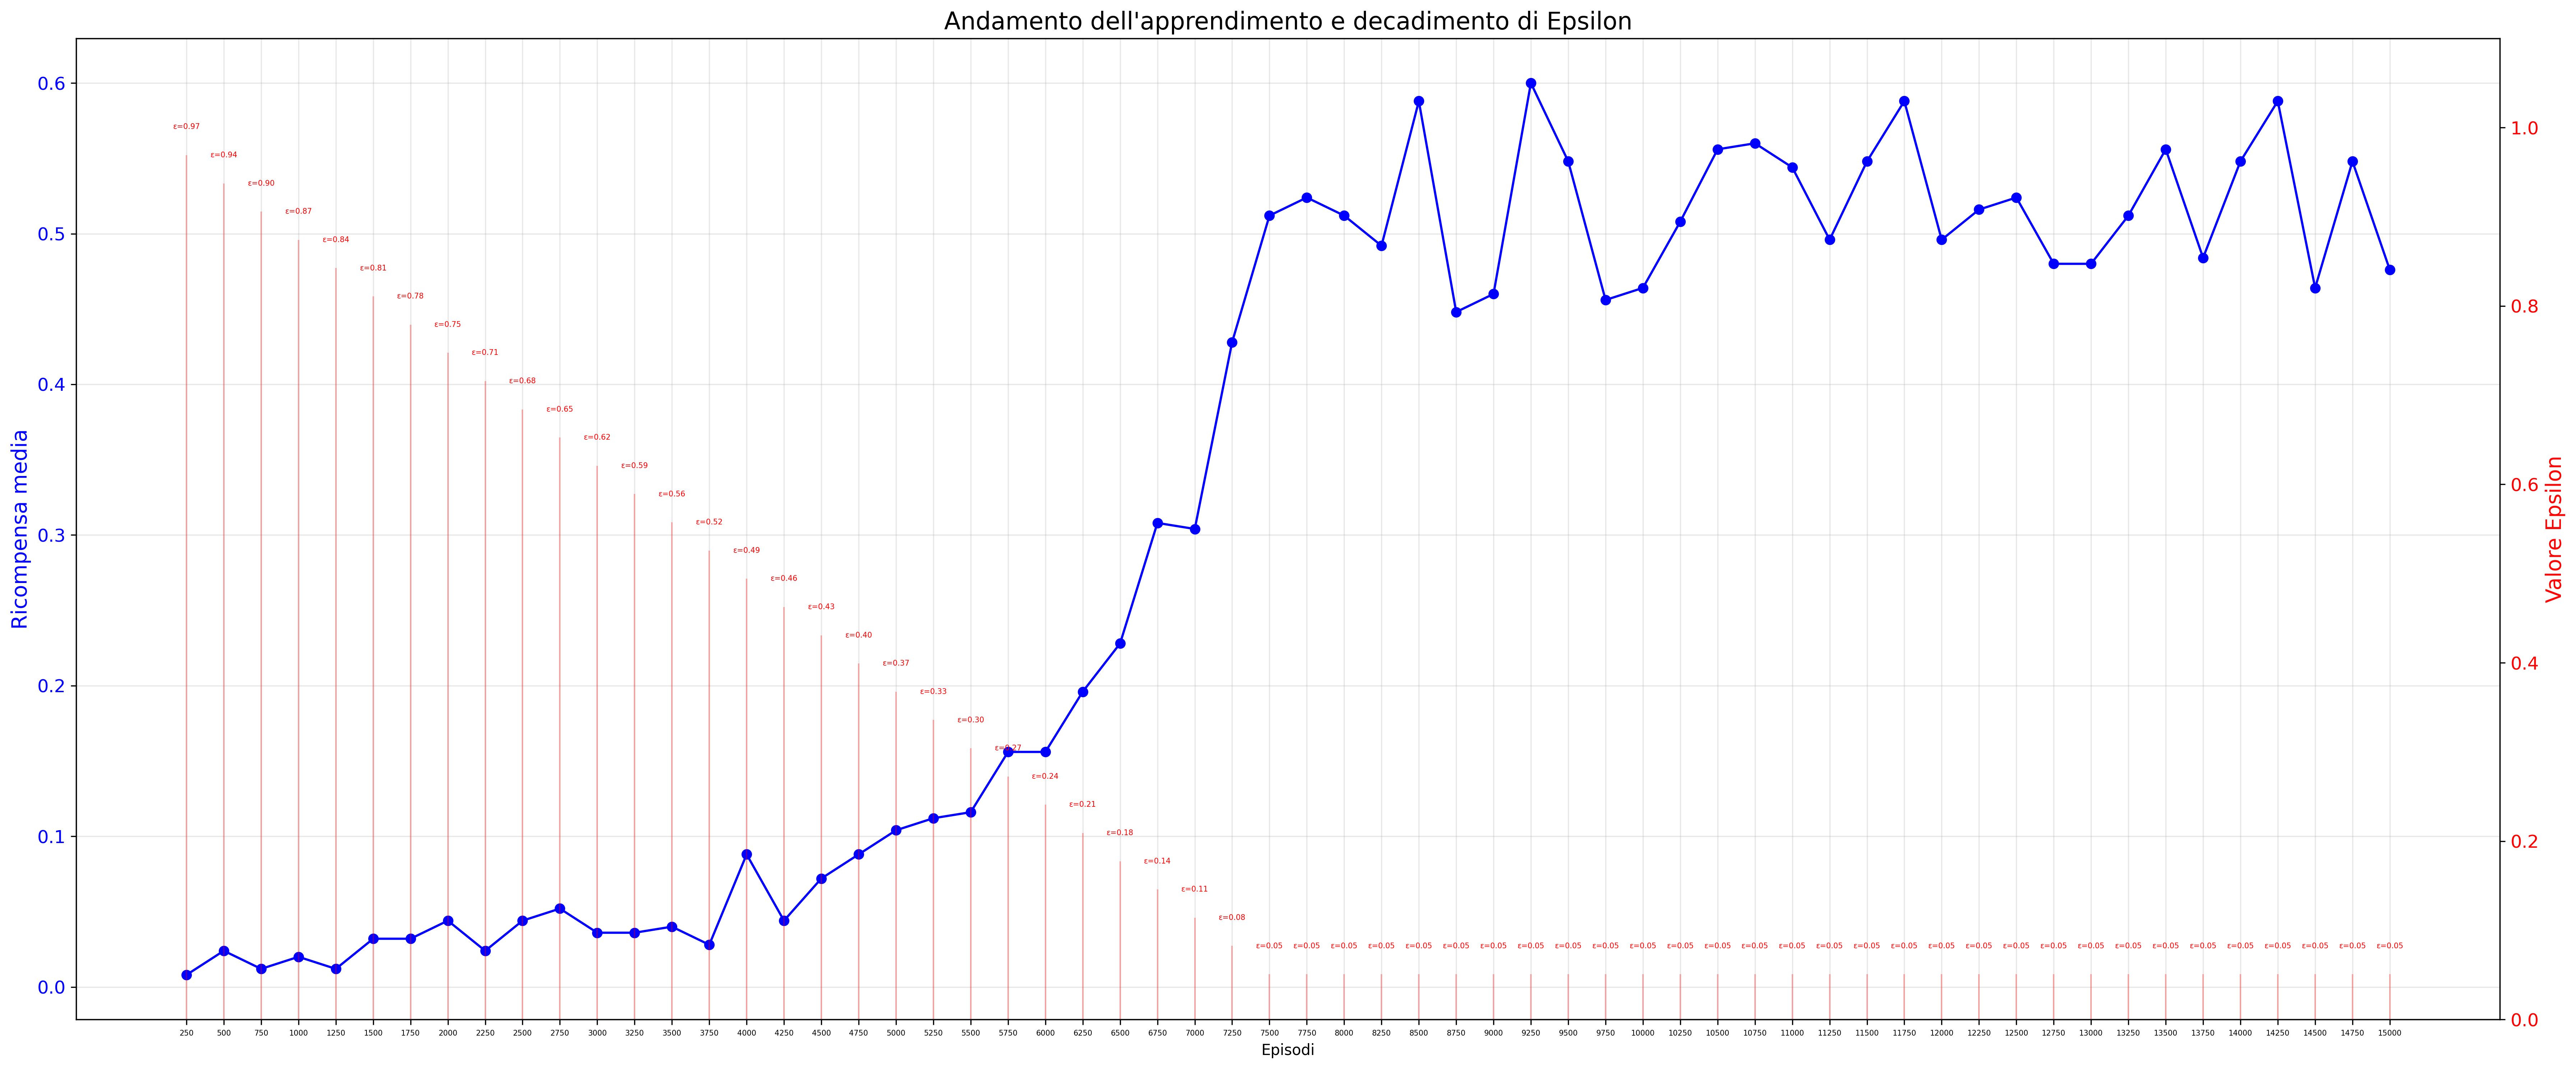
\includegraphics{TQL;lr=0.1;nep=15000;eps=1.0;fineps=0.05;eps_dec=0.00012666666666666666;gam=0.99.png}}
\end{center}

\begin{center}
\centering
\resizebox{\textwidth}{!}{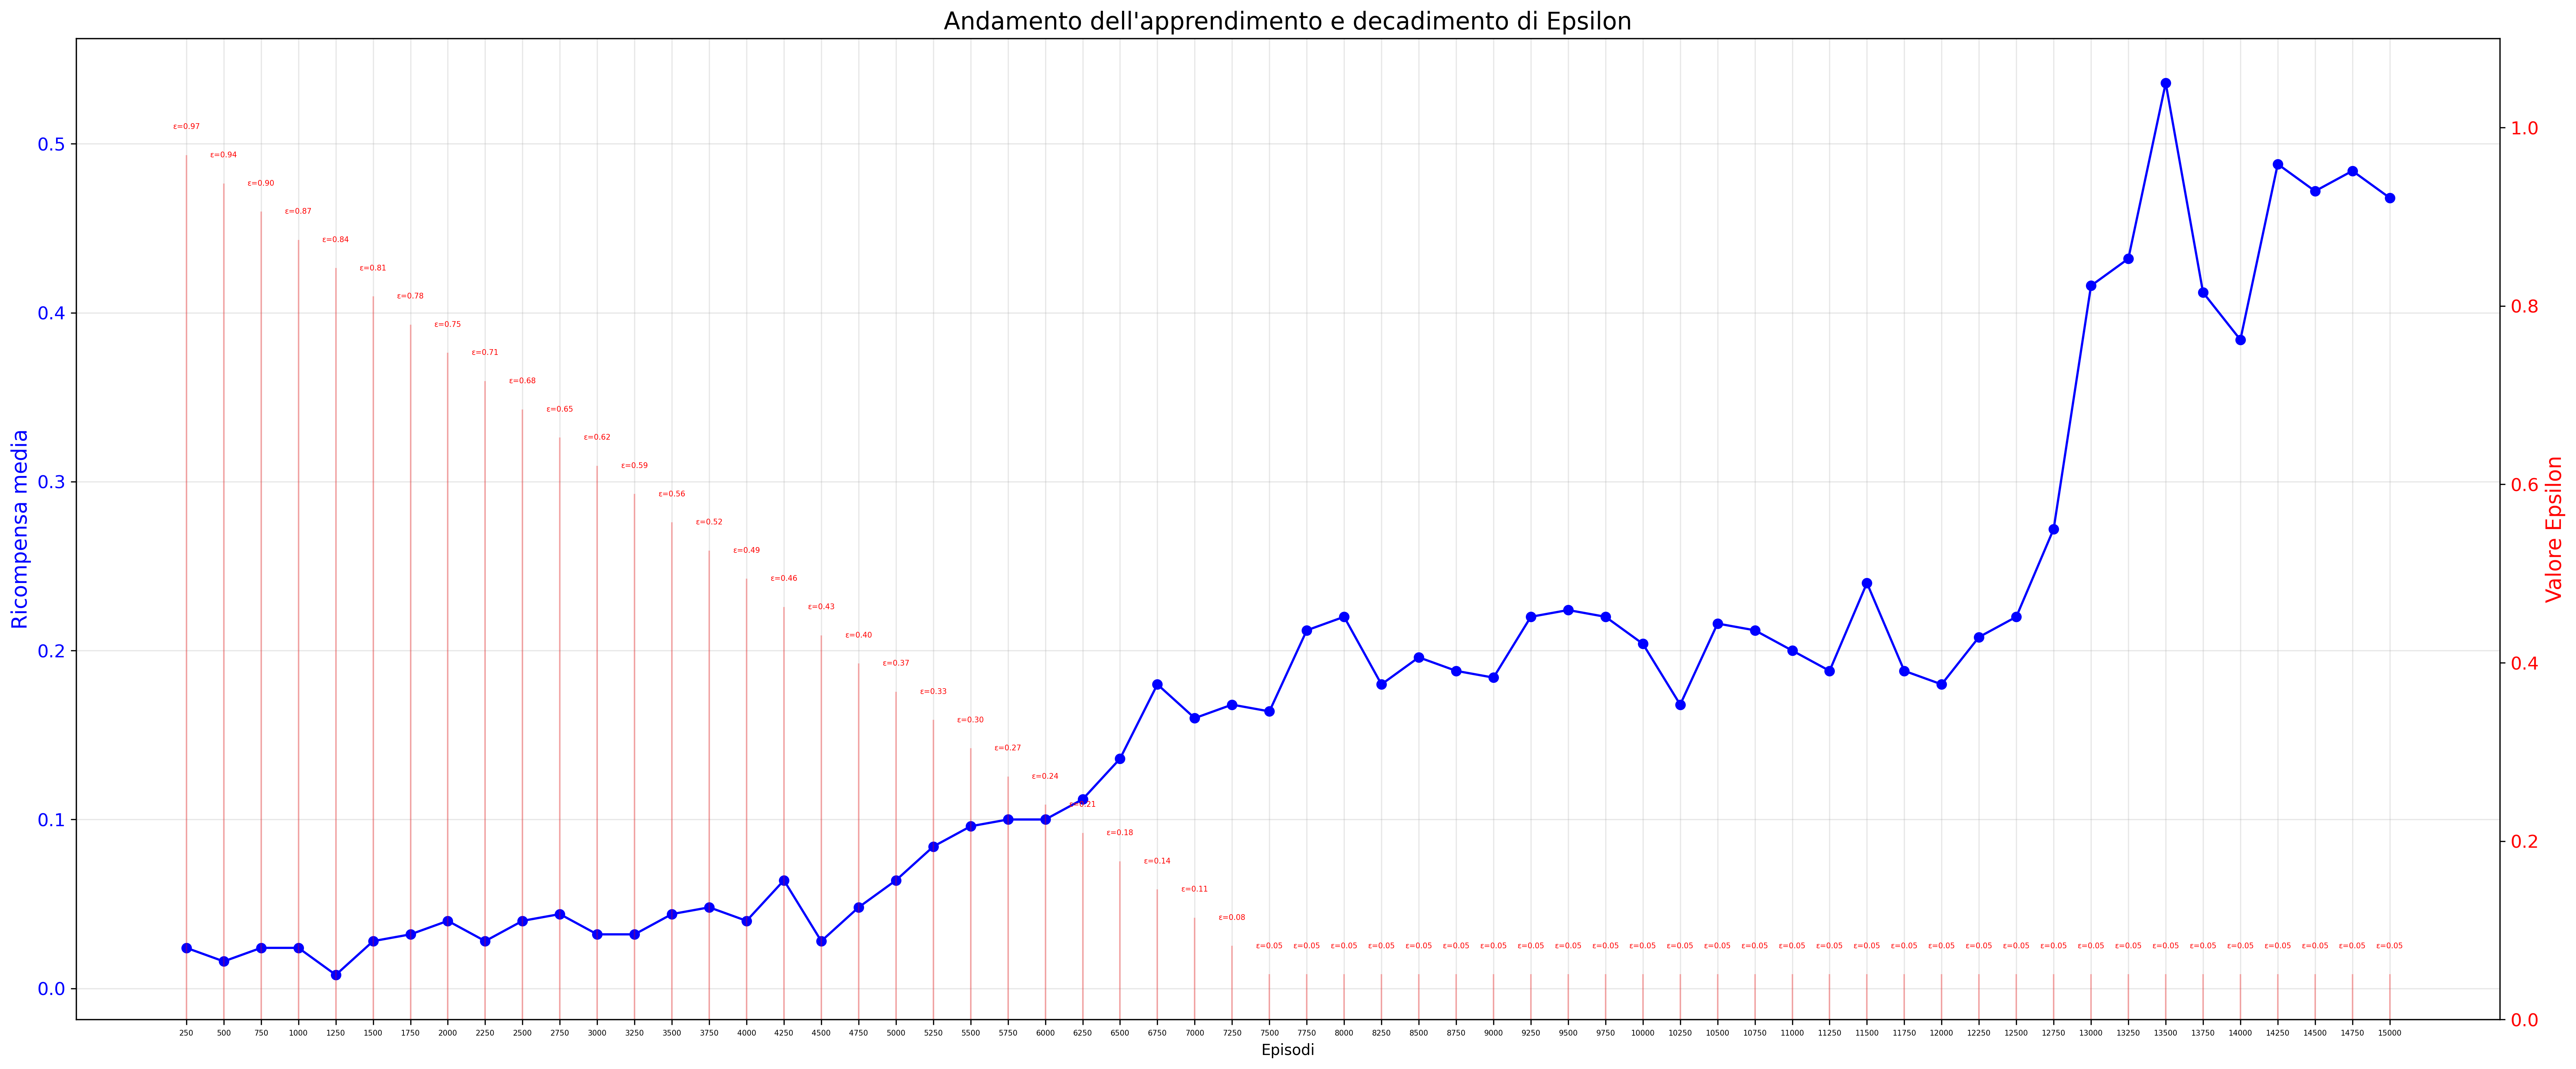
\includegraphics{TQL;lr=0.01;nep=15000;eps=1.0;fineps=0.05;eps_dec=0.00012666666666666666;gam=0.99.png}}
\end{center}

\begin{center}
\centering
\resizebox{\textwidth}{!}{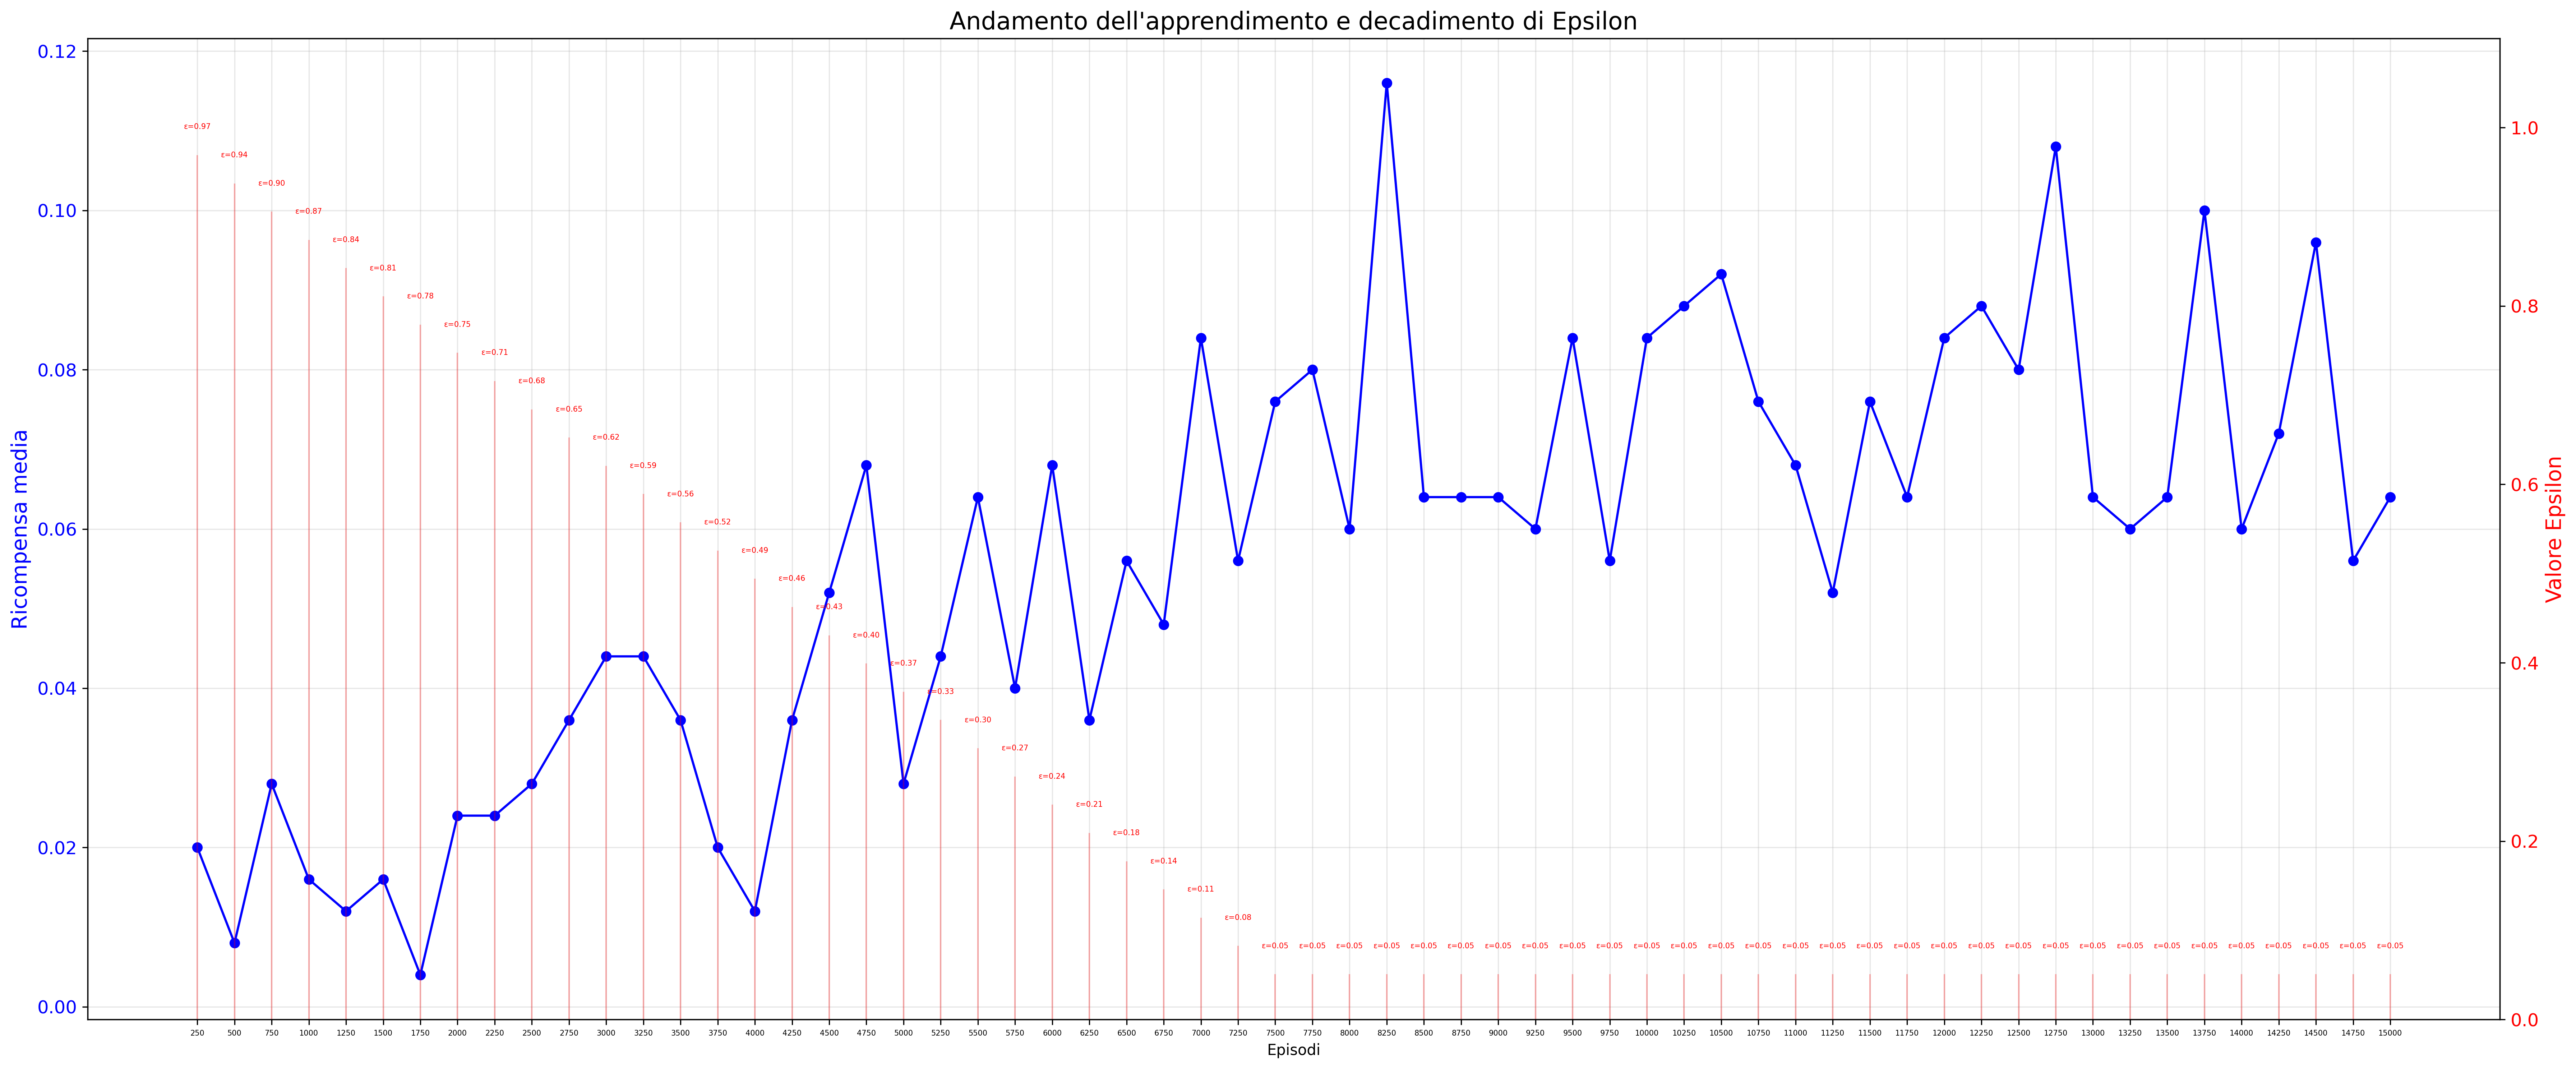
\includegraphics{TQL;lr=0.001;nep=15000;eps=1.0;fineps=0.05;eps_dec=0.00012666666666666666;gam=0.99.png}}
\end{center}

\clearpage


In terms of convergence time, the first solution (with a learning rate of 0.1) is the best, reaching convergence at around episode 7500.
\\
The second configuration reaches a convergence at episode 13000, while the third configuration converges at episode 8000.
\\
In terms of average cumulative reward at convergence, the first solution again performs the best, achieving a reward of 1 (reaching the goal) in 72.6\% of the episodes during the testing phase.
\\
The second solution has an average success rate of 59.6\%, while the third solution performs poorly, with an average success rate of only 6.2\% over the 500 testing episodes.

\subsubsection{Conclusions}

So, in conclusion, I would say that in the case of Tabular Q-learning in a non deterministic environment, the best configuration found is the following one:
\begin{itemize}
\item[--] $\alpha$= 0.1
\item[--] $\epsilon$ decay= 0.000126
\item[--] initial $\epsilon$ = 1
\item[--] final $\epsilon$ = 0.05
\item[--] gamma = 0.99
\end{itemize}


Bringing an average cumulative reward of 0.726 and converging in about 7500 episodes.



\section{Deep Q Network}

\subsection{Solution adopted}

\begin{center}
\centering
\resizebox{\textwidth}{!}{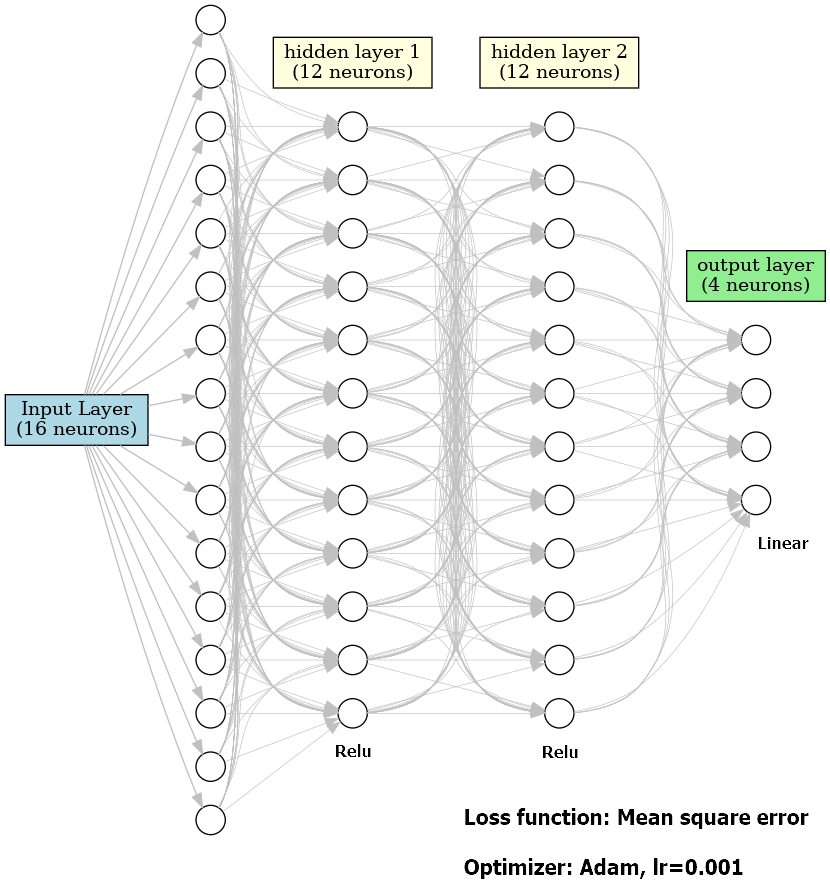
\includegraphics{NN_architecture.png}}
\end{center}

\clearpage

I have used tensorflow with keras for bulding a feedforward neural network for solving the Frozen Lake environment, using always the non deterministic Q learning technique.
\\
These are the characteristics of the network:
\begin{itemize}
\item[--] Feedforward neural network
\item[--] Width is 16, cause the number of neurons of the input layer
\item[--] Depth is 2, because we have 2 hidden layers
\item[--] The neurons are fully connected in a Dense way (each neuron is connected with all the following neurons)
\item[--] The activation function of the hidden layers is the Relu (Rectified linear units)
\item[--] The activation function of the output layer is the Linear (Identity function)
\item[--] The loss function used is the Mean Square Error
\item[--] The optimizer used is Adam, with a learning rate of 0.001
\item[--] The number of training episode is 15000
\item[--] The average cumulative reward is calculated over a range of 250 episodes
\item[--] The number of test episodes is 500
\item[--] The mini-batch size is 64
\end{itemize}

The number of neurons in the neural network, and the type of connection (Dense), achieves the presence of 384 weight parameters.
\\
\\
\textbf{OPTIMIZER}
\\
The optimizers (which in this case is Adam), have the goal of adapting the learning rate value (starting from 0.001 in this case) with respect to the current iteration in the training phase; this is done because through the gradient of the loss function at each iteration, we have to perform an adjustment to the weights that contribute to the error.
\\
We want the adjustments to be bigger in the first iterations and lower in the later ones, and this is achieved by controlling how the learning rate influences the weight updates during the correction phase, which is the optimizers goal.
\\
\\
\textbf{LOSS FUNCTION}
\\
The loss function (which in this case is the mse), has the goal of calculate the difference between a predicted value and the actual value from the training dataset.
\\
\\
\textbf{ACTIVATION FUNCTION}
\\
The activation functions (Which in this case are the Relu: g($\alpha$) = max(0,$\alpha$) and the Linear: identity function) are the functions which applies to the weighted sum of the inputs to each neuron, giving the output.
\\
In the hidden layers they are not linear and aim to introduce non linearity, in order to be able to capture the non linear relationship between the states and their optimal Q values.
\\
To be precise, for computing the gradient on the loss function for correcting the weight's values, we are computing it also on the activation function, but we have no troubles cause the non derivability at the point x=0 (in the case of relu), because is almost impossible that we reach exactly that point during the training phase.
\\
\\
\textbf{REPLY BUFFER}
\\
In reinforcement learning it is a data structure commonly used in algorithms like Q-learning.
\\
It stores tuples of the form (state, action, reward, next state) that are generated at each step during the training phase.
\\
When the neural network trains at each episode, it updates the model using only a sample (in this case, of size mini-batch = 64) from the total training data stored in the replay buffer. 
\\
This approach speeds up training by avoiding the need to train on the entire dataset at each iteration, which grows with each step.
\\
It is important to note that the values stored in the tuples are the ones needed and used to update the Q-values, which are then used for training.


\subsection{Metric results}


\subsubsection{Changing the epsilon decay}


These are the common hyper parameters for the runs:
\begin{itemize}
\item[--] $\alpha$= 0.1
\item[--] initial $\epsilon$ = 1
\item[--] final $\epsilon$ = 0.05
\item[--] gamma = 0.99
\end{itemize}

From the first plot to the third, the $\epsilon$ decay rate is increased as follows:

\begin{itemize}
\item[--] The first brings $\epsilon$ to its minimum value at 7/8 of the episodes.
\item[--] The second brings $\epsilon$ to the minimum at 3/4 of the episodes.
\item[--] The last one brings $\epsilon$ to the minimum at 1/2 of the total episodes.
\end{itemize}


\begin{center}
\centering
\resizebox{\textwidth}{!}{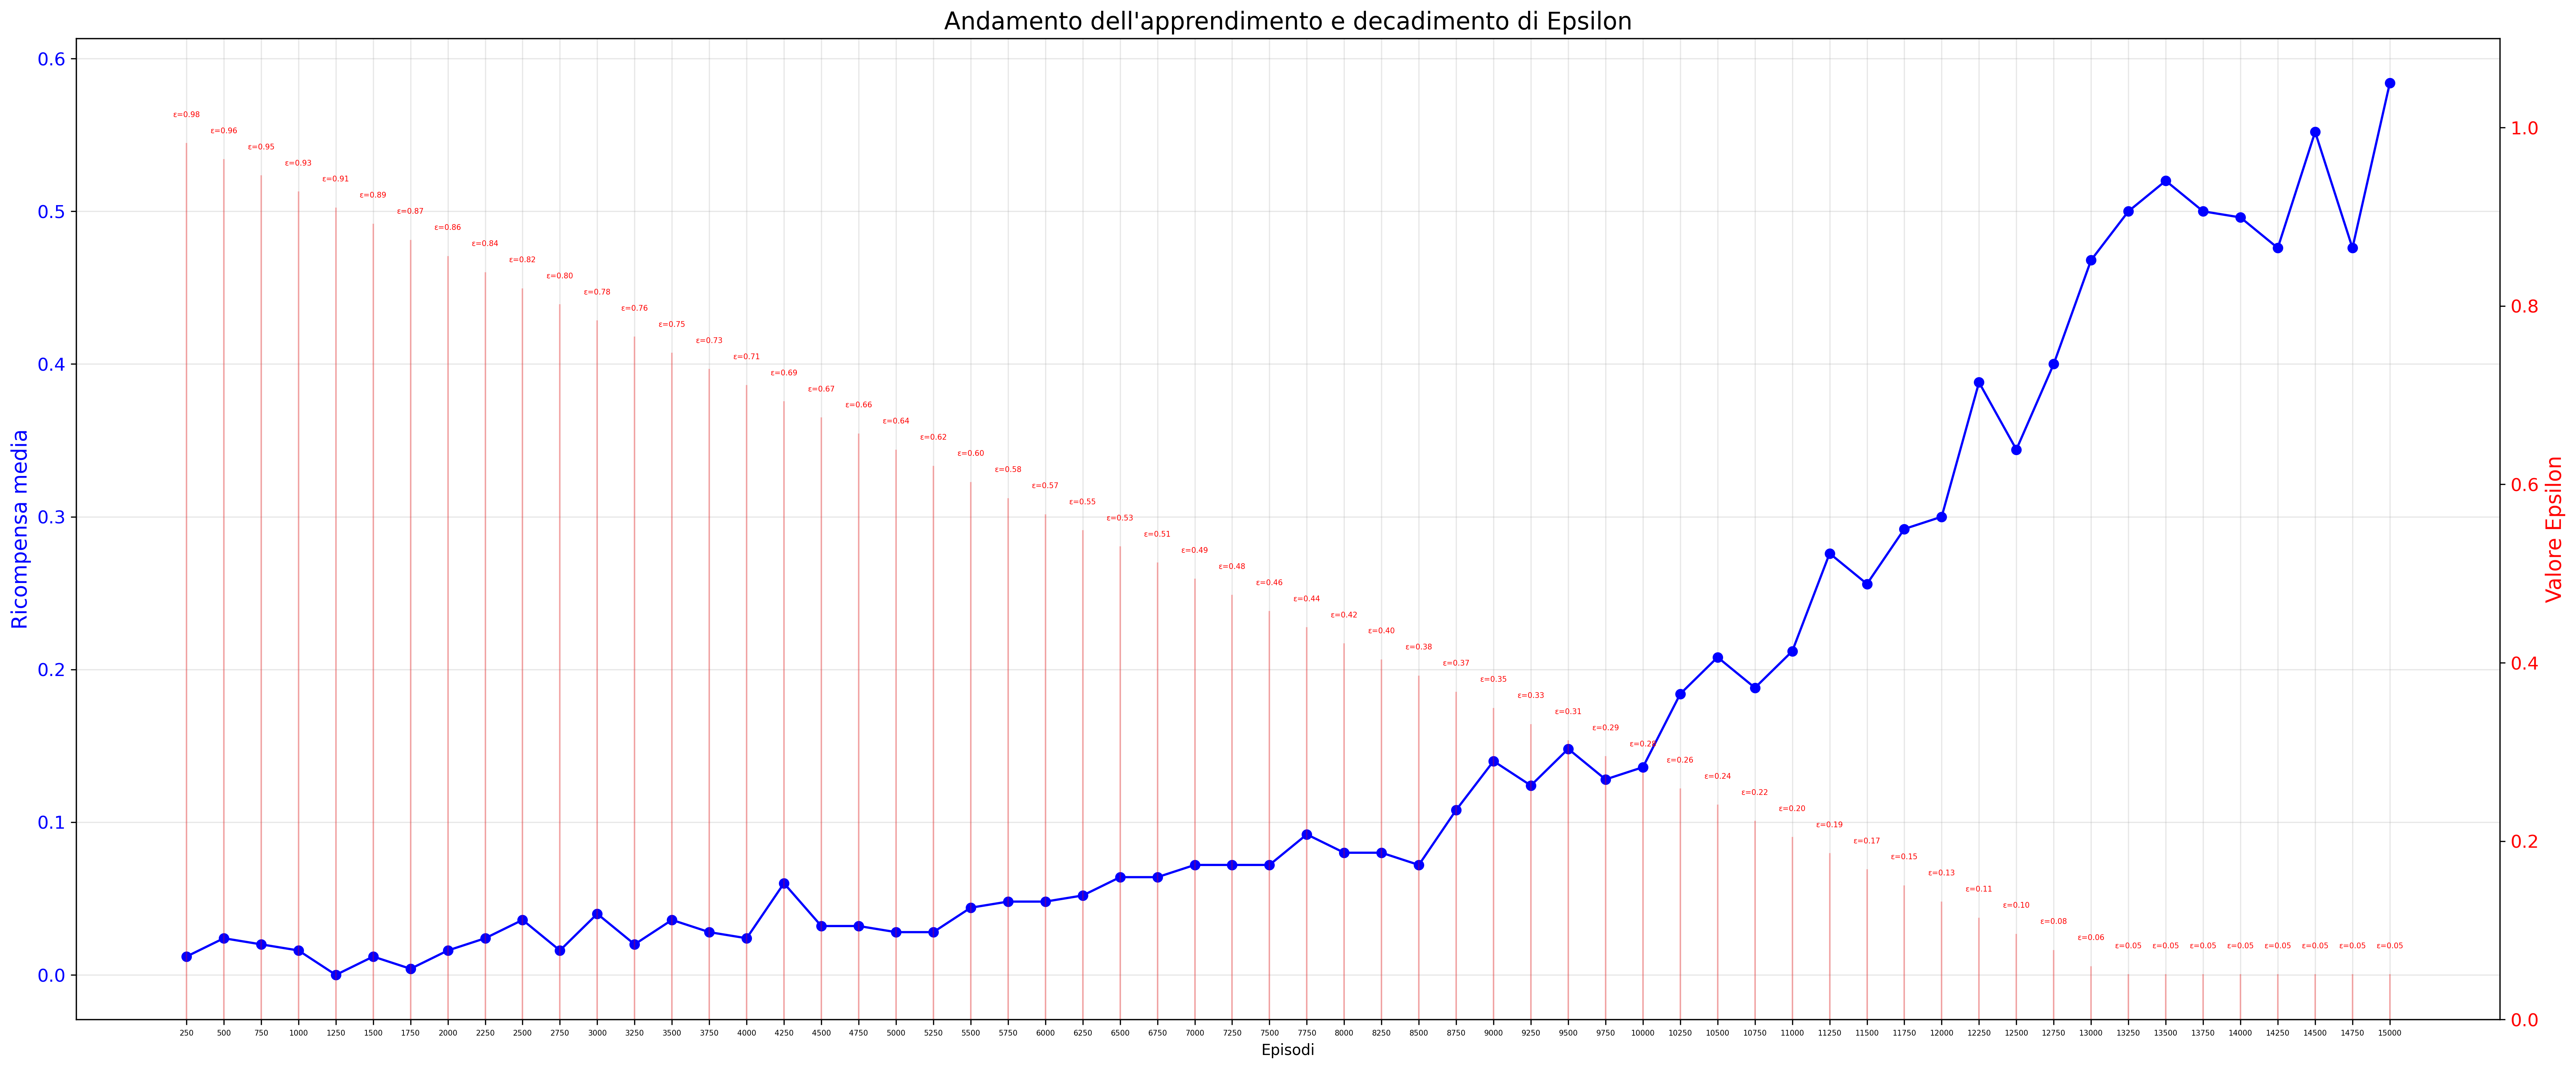
\includegraphics{DQN;lr=0.1;nep=15000;eps=1.0;fineps=0.05;eps_dec=7.238095238095238e-05;gam=0.99.png}}
\end{center}

\begin{center}
\centering
\resizebox{\textwidth}{!}{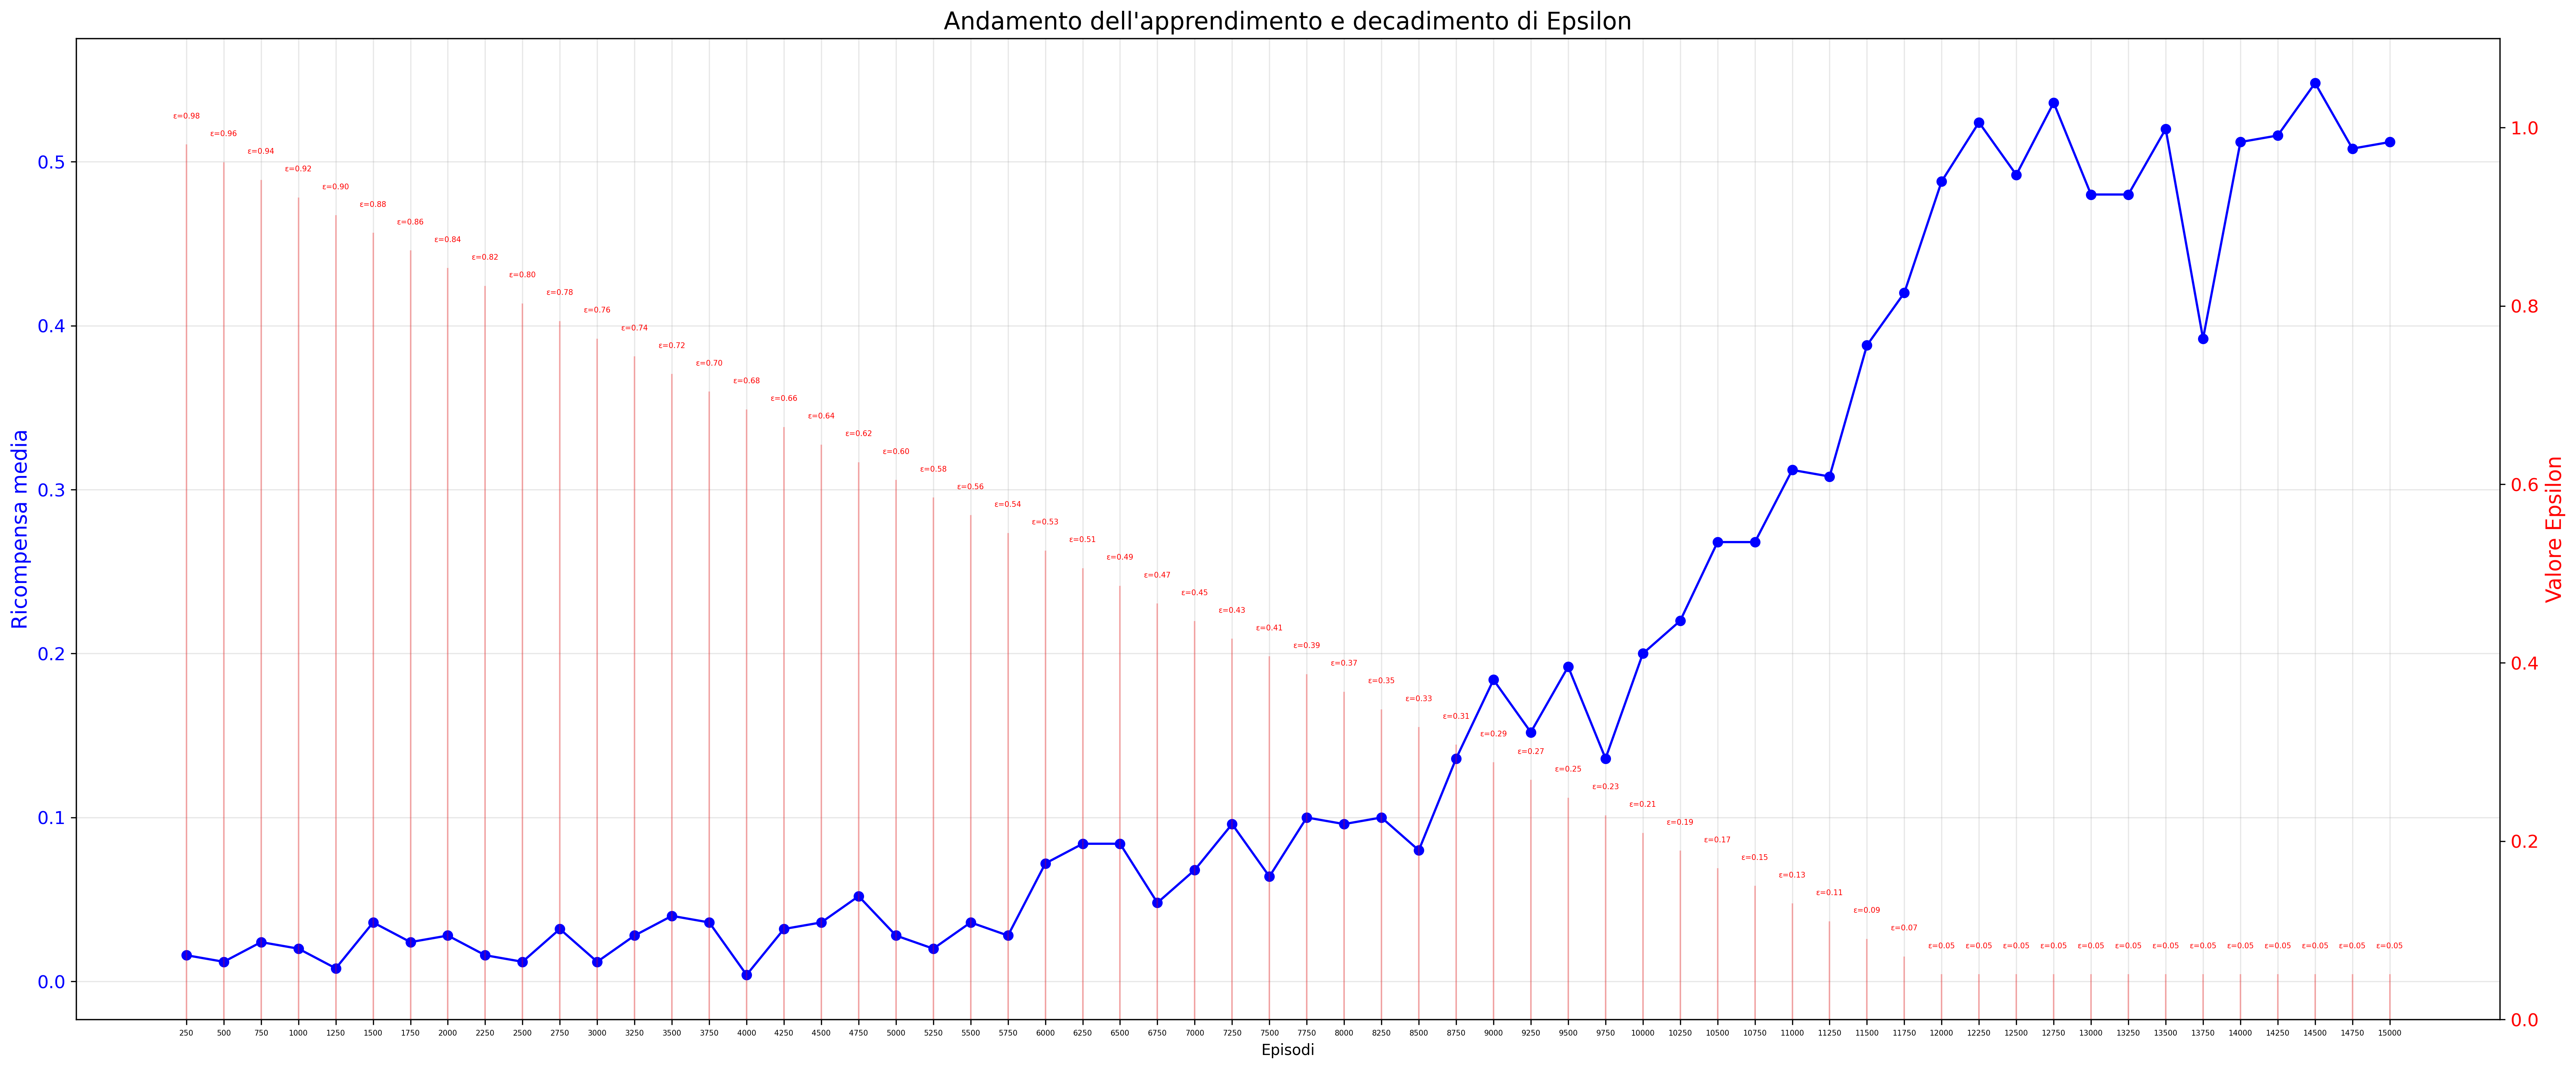
\includegraphics{DQN;lr=0.1;nep=15000;eps=1.0;fineps=0.05;eps_dec=7.916666666666666e-05;gam=0.99.png}}
\end{center}

\begin{center}
\centering
\resizebox{\textwidth}{!}{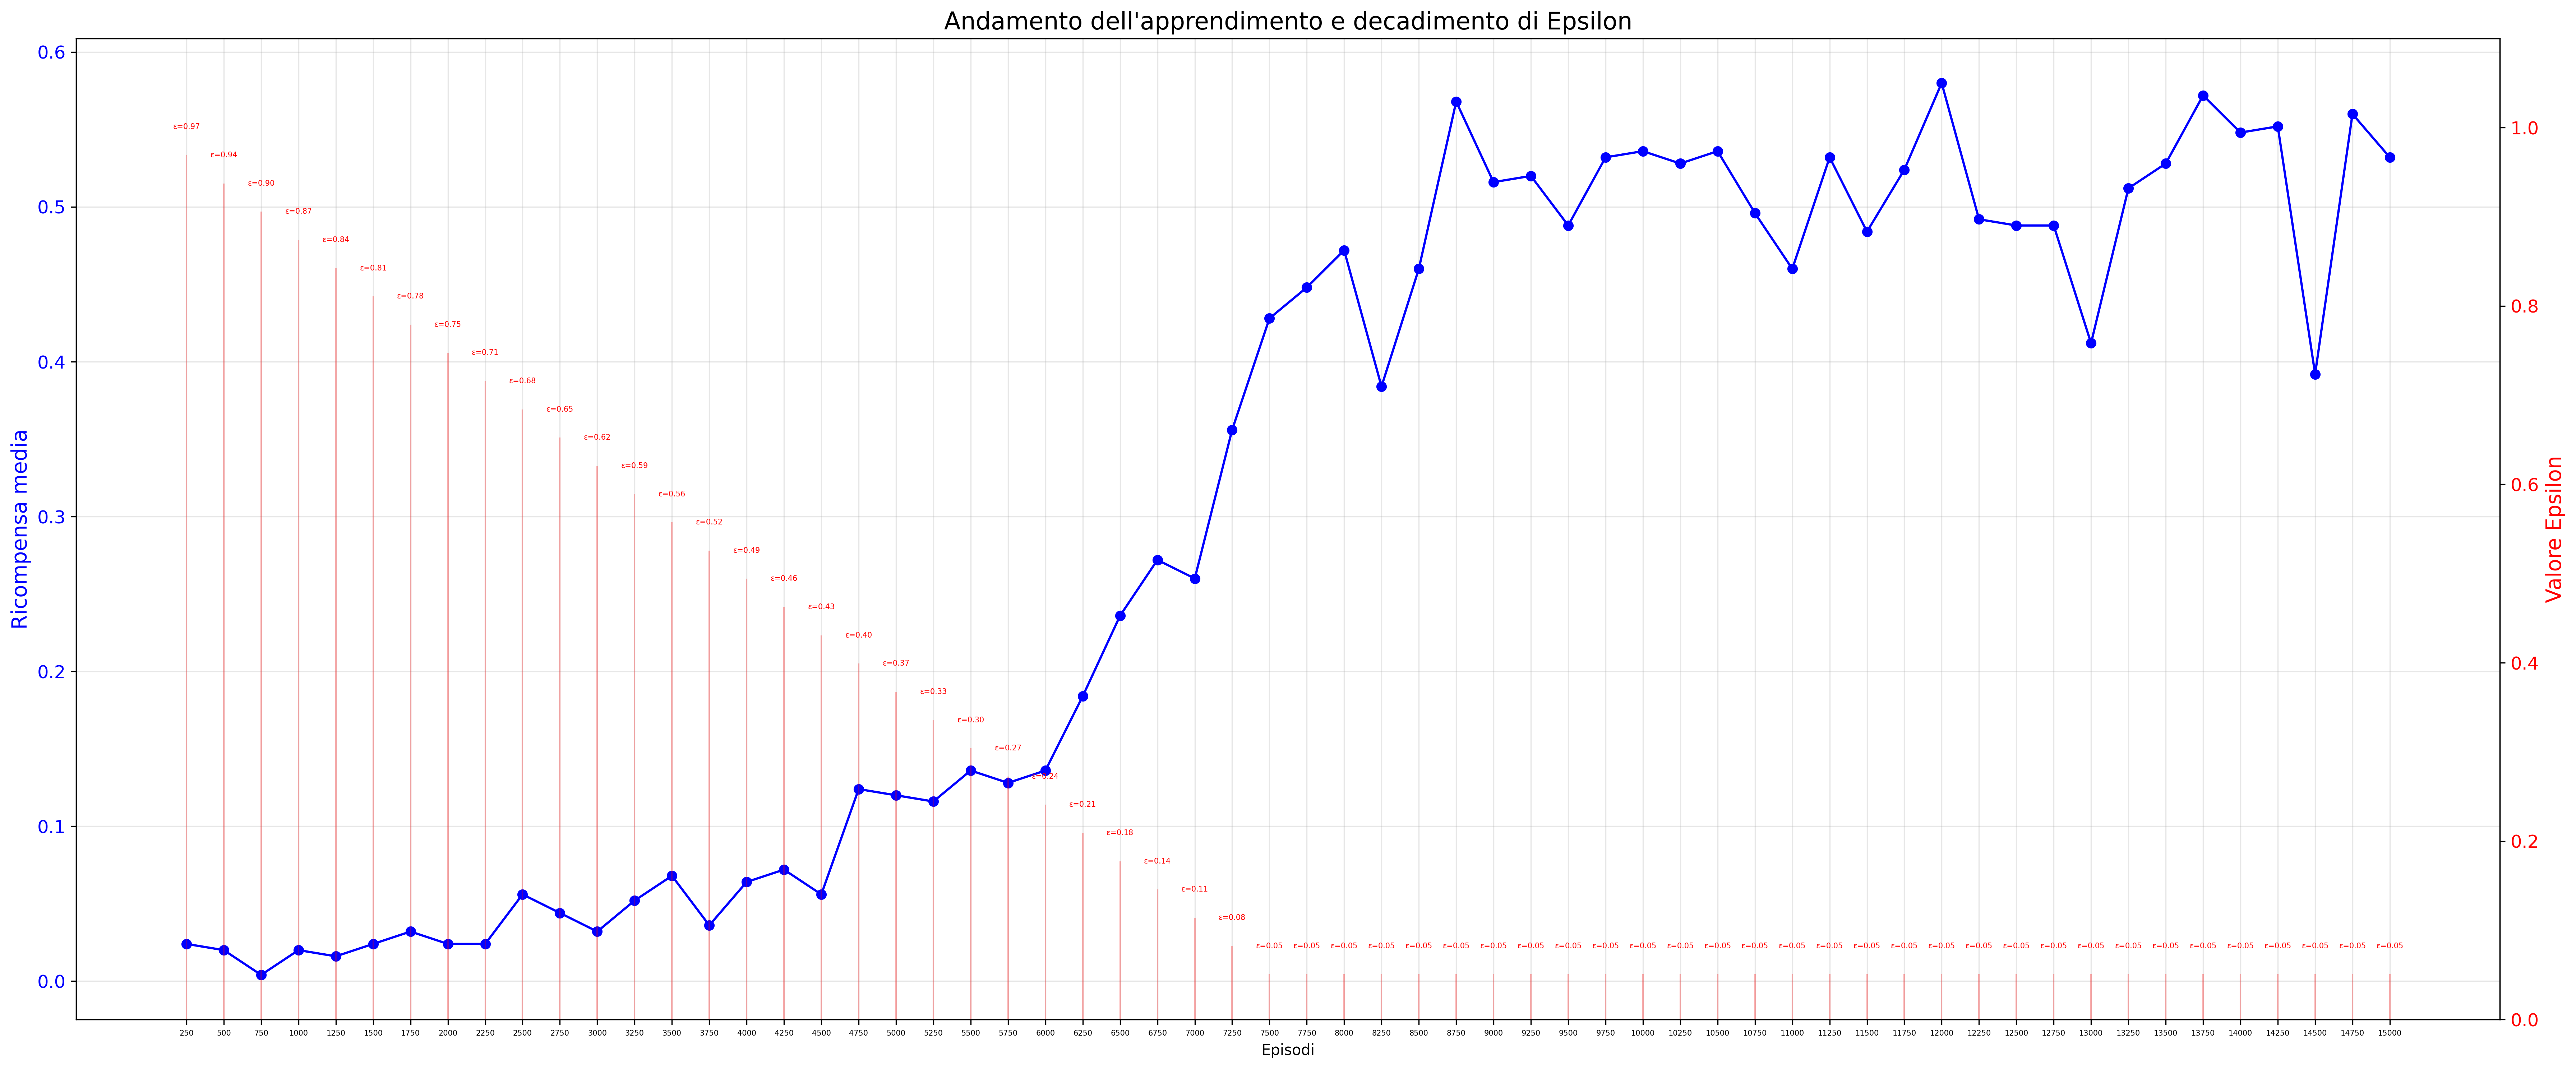
\includegraphics{DQN;lr=0.1;nep=15000;eps=1.0;fineps=0.05;eps_dec=0.00012666666666666666;gam=0.99.png}}
\end{center}

\clearpage


In the first configuration (with $\epsilon$ which goes to the minimum at 7/8 of the episodes) the convergence is achieved almost at the 13250 episode.
\\
In the second, instead, the convergence is achieved at 12250 episodes, then the third configuration is the best, converging on the 9000 episode.
\\
If we focus on the average cumulative reward at convergence, we could say that the first configuration is slightly better, achieving a success rate of the 52\%, against a 50\% achieved by the other two configurations.
\\
Now, considering the testing phase, which is done on 500 epsiodes: the second and third configurations are the best, having a 73.4\% of success rate, then the first achieves the 72.6\%.
\\
So, we can conclude that in terms of cumulative rewards, all the three possibilities has slightly the same performances, so I would say that the third configuration is the best, due to its faster convergence time.


\subsubsection{Changing the learning rate}


These are the common hyper parameters for the runs:
\begin{itemize}
\item[--] $\epsilon$ decay= 0.000126
\item[--] initial $\epsilon$ = 1
\item[--] final $\epsilon$ = 0.05
\item[--] gamma = 0.99
\end{itemize}

From the first plot to the third, the $\alpha$ value assumes the following values :
\begin{itemize}
\item[--] The first sets $\alpha$ to 0.1
\item[--] The second sets $\alpha$ to 0.01
\item[--] The third sets $\alpha$ to 0.001
\end{itemize}

\clearpage


\begin{center}
\centering
\resizebox{\textwidth}{!}{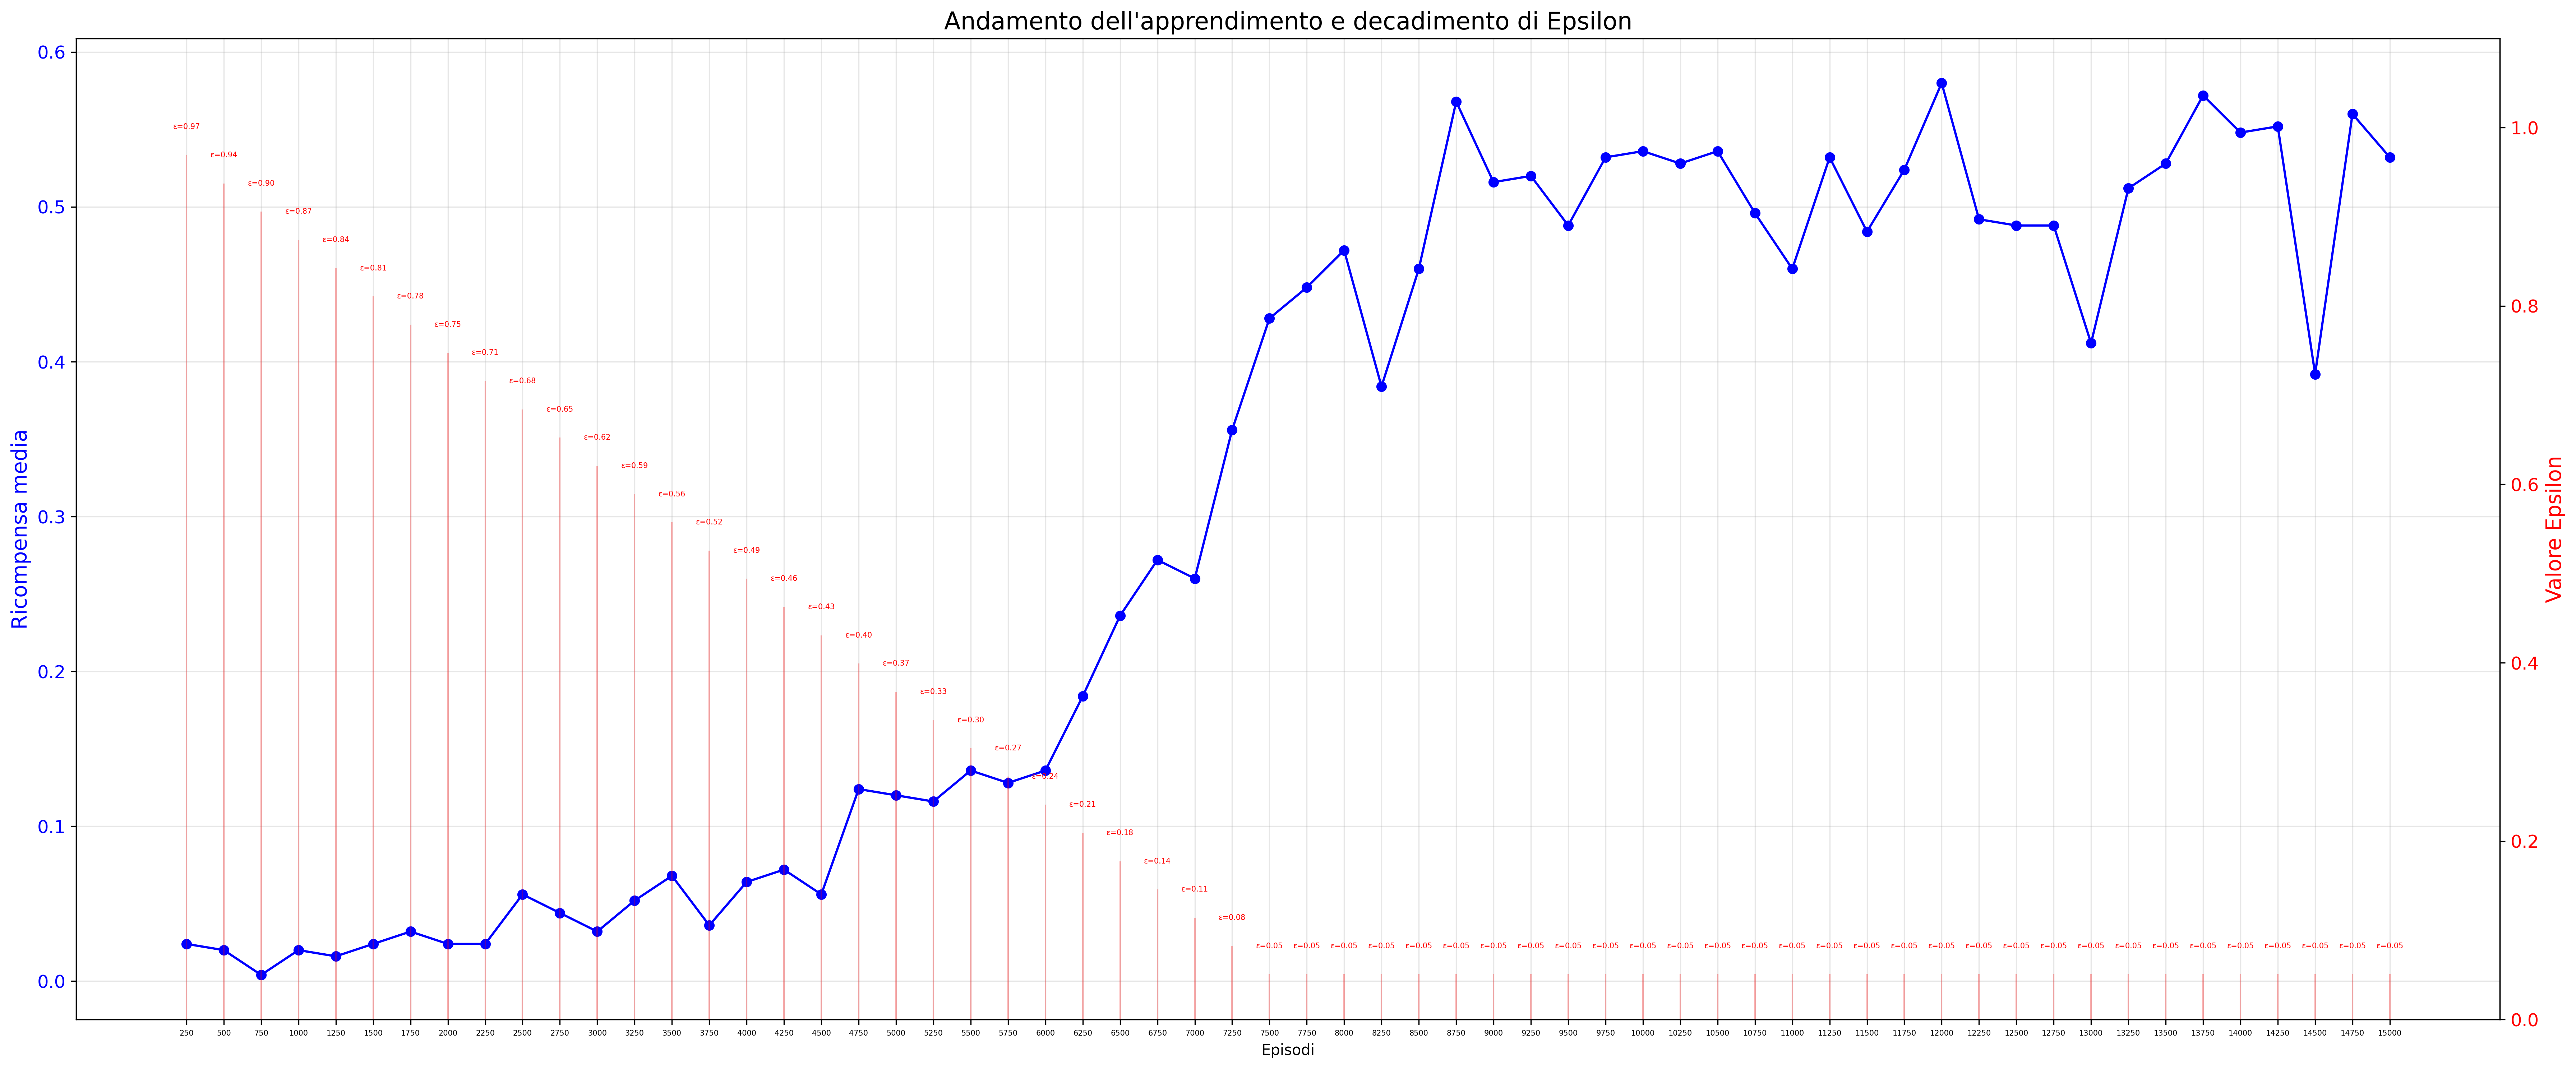
\includegraphics{DQN;lr=0.1;nep=15000;eps=1.0;fineps=0.05;eps_dec=0.00012666666666666666;gam=0.99.png}}
\end{center}

\begin{center}
\centering
\resizebox{\textwidth}{!}{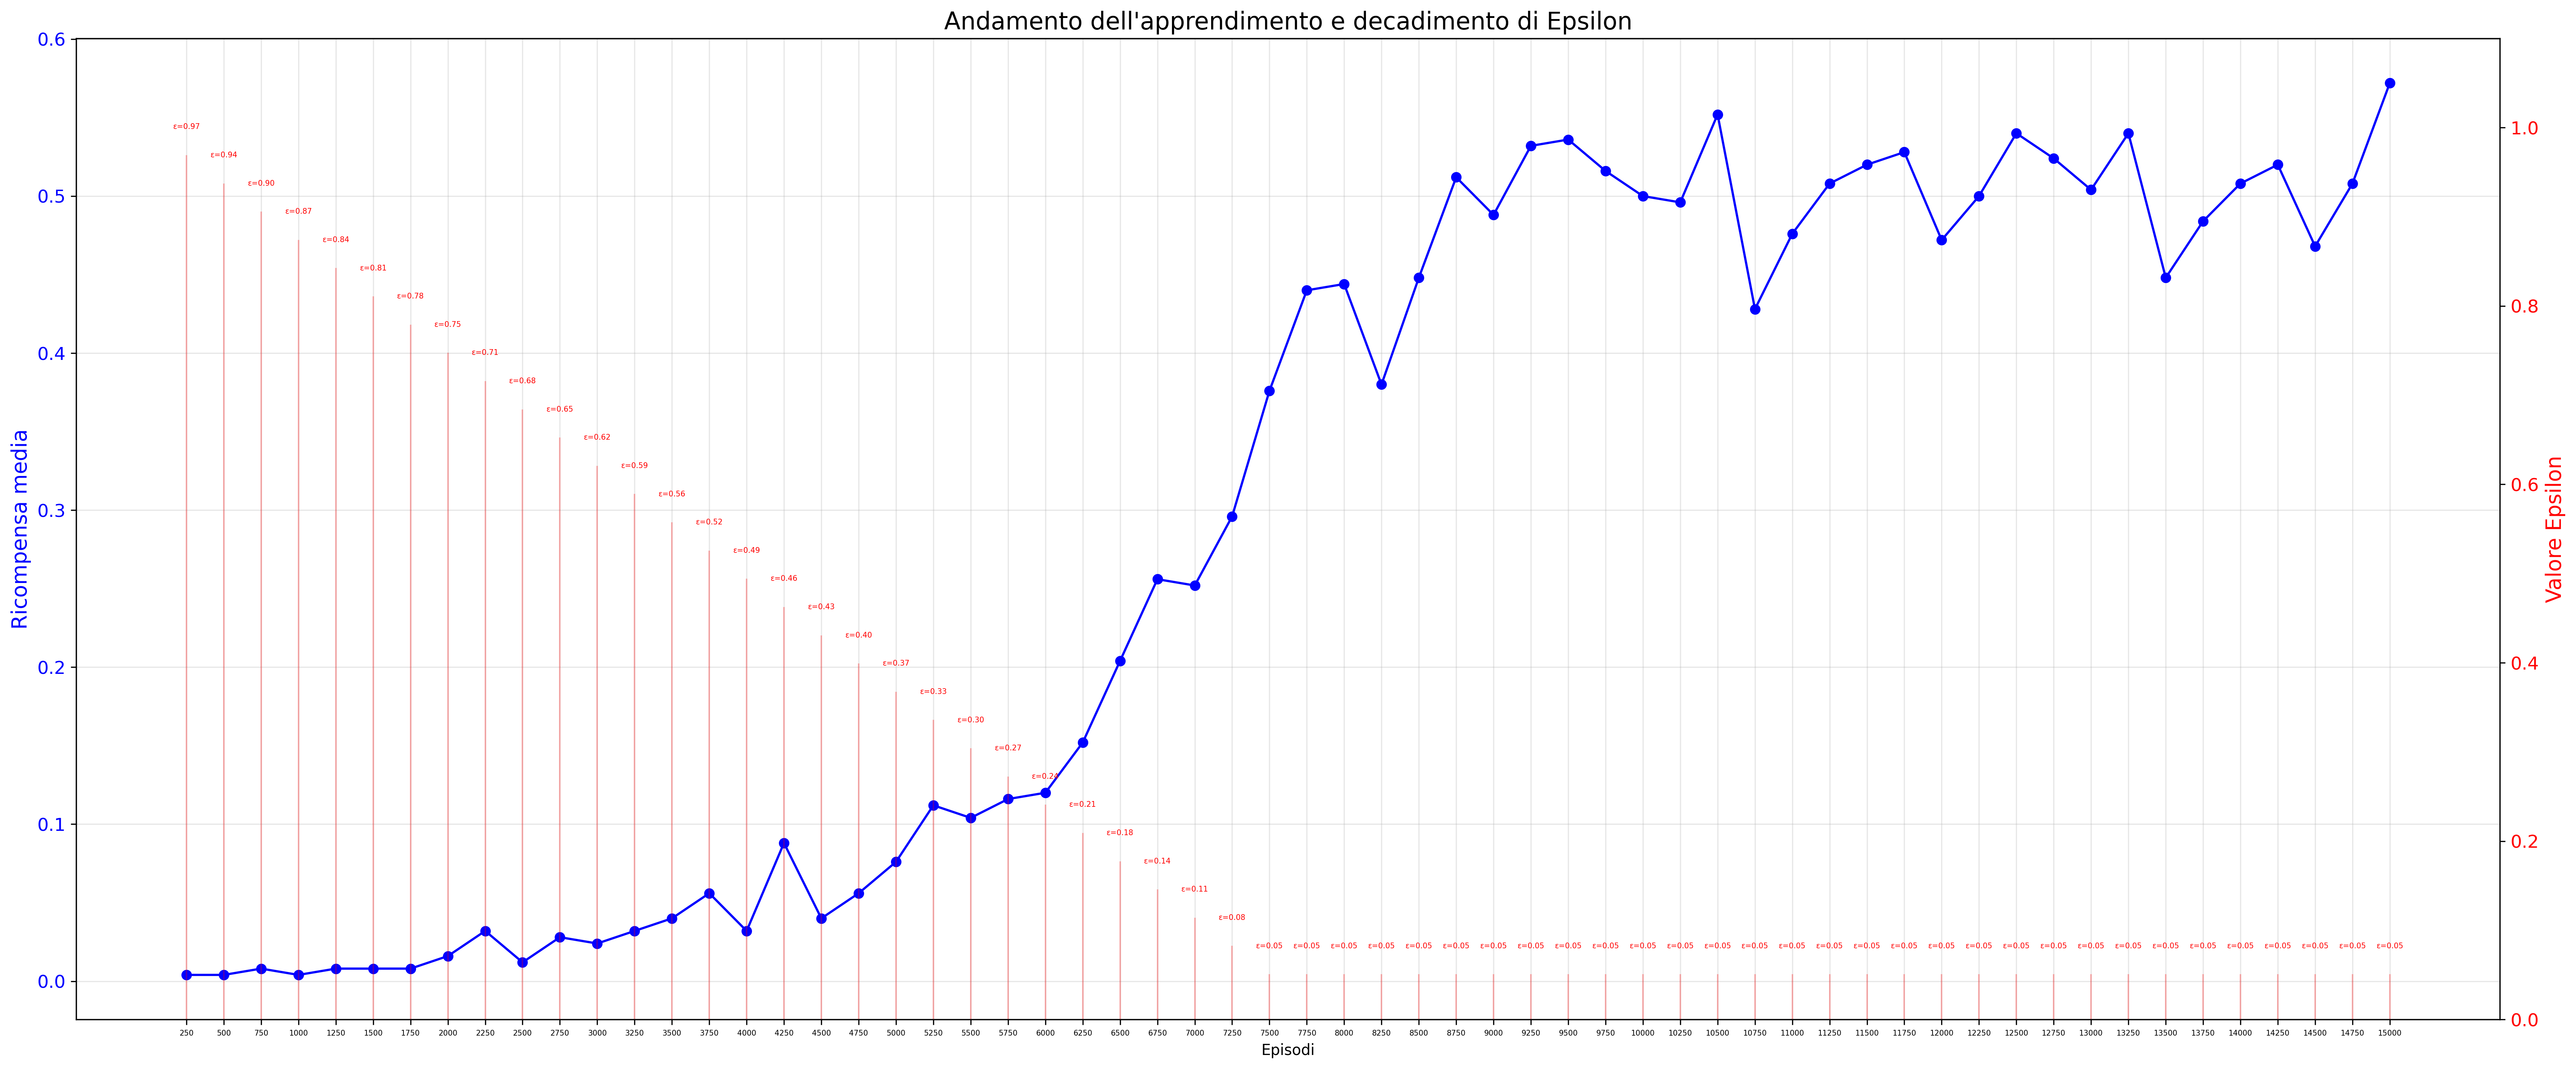
\includegraphics{DQN;lr=0.01;nep=15000;eps=1.0;fineps=0.05;eps_dec=0.00012666666666666666;gam=0.99.png}}
\end{center}

\begin{center}
\centering
\resizebox{\textwidth}{!}{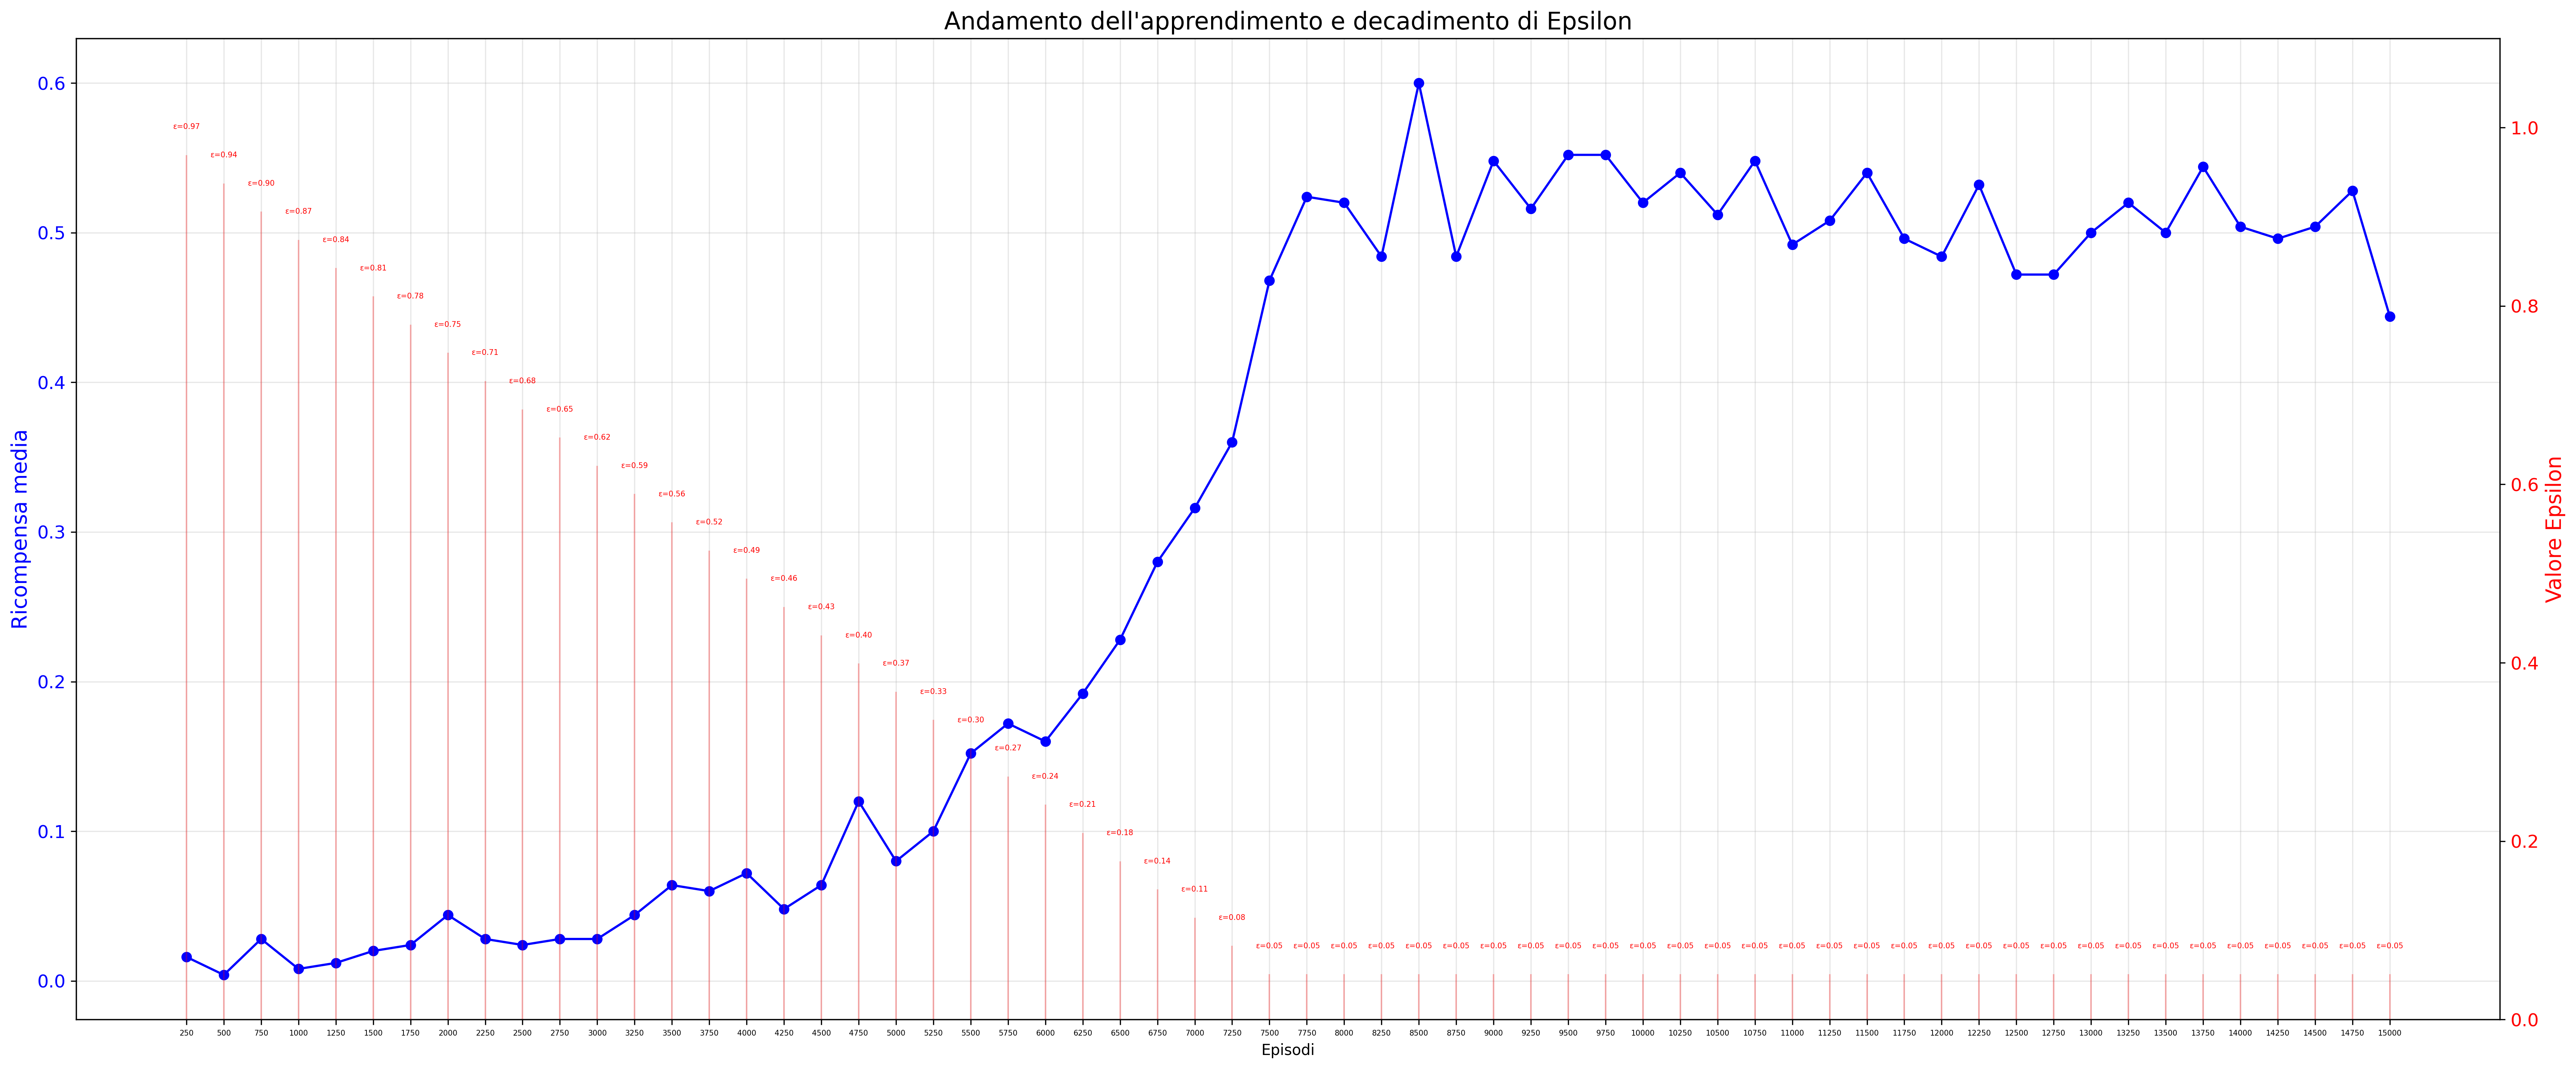
\includegraphics{DQN;lr=0.001;nep=15000;eps=1.0;fineps=0.05;eps_dec=0.00012666666666666666;gam=0.99.png}}
\end{center}

\clearpage


Considering the convergence time, the third configuration is the best, achieving that after 7750 episodes, but also the other ones don't behave badly, given that the first configuration converge after 
9000 epsiodes and the second one after 8750.
\\
With respect to the average cumulative reward at convergence aspect, both the first and the second one brings a success rate of 50\%, then the third one of 53\%.
\\
In terms of reward obtained in the testing phase, the second configuration is the best, bringing an average success rate of 75.2\%, instead, the first one brings the 73.4\% and the third,
which is slightly the worst one, bring success rate of the 72\%.
\\
In conclusion, I would say that both the three possibilities are similar in terms of performance, with the second one that takes some more episodes wrt the third one, but brings the best reward on the testing phase.


\subsubsection{Conclusions}

So, in conclusion, I would say that in the case of Deep Q Network in a non deterministic environment, the best configuration found is the following one:
\begin{itemize}
\item[--] $\alpha$= 0.01
\item[--] $\epsilon$ decay= 0.000126
\item[--] initial $\epsilon$ = 1
\item[--] final $\epsilon$ = 0.05
\item[--] gamma = 0.99
\end{itemize}

Bringing an average cumulative reward of 0.752 and converging in about 8750 episodes.

\end{document}
